\begin{comment}
\chapter{Systematic Uncertainties}

Systematic uncertainty control is very important to and a highlight of this 
high-precision experiment. To achieve a smaller systematic uncertainty, a
combination of fast-control and slow control was employed, which helped us
to eliminate systematic uncertainties brought by the accelerator to the
beam. Except the uncertainty from the machine, another important source
of systematic undertainties come from detection process, namely the 
acceptance function.

%%%%%%%%%%%%%%%%%%%%%%%%%%%%%%%%%%%%%%%%%%%%%%%%%%%%%%%%%%%%%%%%%%%%%%%%
\section{$Q^2$ and $\theta$}
Physical interpretation of $\CA_{PV}$ requires measurement of precise knowledge
of the scattering angle and corresponding $Q^2$, which were determined using
a watercell target. As we will discuss later, when we run
    from the reconstructed scattering angle $\theta_{lab}$,
Counting mode:
\begin{itemize}
    \item low current
    \item single electron events
    \item tracks 
\end{itemize}
The scattering angle was measured using the watercell target, with the elastic
scattering peak:
\begin{equation}
    \Delta E' = E'_O - E'_H = E\left( \frac{1}{1 + \frac{E(1-\cos\theta)}{M_O}} -
    \frac{1}{1 + \frac{E(1-\cos\theta)}{M_H}} \right)
\end{equation}

\begin{equation}
    Q^2 = 2EE'(1-\cos\theta)
\end{equation}


%%%%%%%%%%%%%%%%%%%%%%%%%%%%%%%%%%%%%%%%%%%%%%%%%%%%%%%%%%%%%%%%%%%%%%%%
\section{Carbon Contamination in PREX-II}
The Pb foil is not good thermal conductivity, which limits the highest current
we can apply. To help dissipate the heat produced
by electron bombarment, auxiliary meterials -- the Diamond foils, which are 
excellent thermal conductivity are used. Besides, C12 is isoscalar, and spin-0 
nucleus, whose PV asymmetry is well-measured (FIXME), so the background is 
well-understood. Even so, the highest current is only $70 \ \mu A$.

The Pb208 foil is $0.5\ mm$ thick, each diamond foil is half the thickness 

For CREX, Ca48 has good thermal conductivity, so the current can go up to $150\ \mu A$
the contamination is mainly Ca40 ($\sim 4\%$ FIXME), which is also isoscalar
and spin-0 nucleus, so benign background
\end{comment}

%%%%%%%%%%%%%%%%%%%%%%%%%%%%%%%%%%%%%%%%%%%%%%%%%%%%%%%%%%%%%%%%%%%%%%%%
\section{Accptance Function}
As we said before, the spectrometer acceptance was mainly defined by the Q1 
collimator, but other devices may also have affections on it. And the accepted
area was not tiny ($0.00377 \ sr$), not every point within the acceptance had
the same detection efficiency and cross section asymmetry, therefore what
we measured was actually the average asymmetry over the acceptance:
\begin{equation}
    \CA_{mea} = \frac{\int d\theta \sin\theta A(\theta) \frac{d\sigma}{d\Omega} \epsilon(\theta)}{\int d\theta \sin\theta \frac{d\sigma}{d\Omega} \epsilon(\theta)}
    \label{eq:acceptance_function}
\end{equation}
Here $\epsilon(\theta)$ is the aceeptance function, which is defined as
the ratio of electrons that reach the main detector over all scattered
electrons, which depends on the scattering angle $\theta$:
\begin{equation}
    \epsilon(\theta) = \frac{N_{det}(\theta)}{N_{sca}}
    \label{eq:acceptance_definition}
\end{equation}

From Eq. \ref{eq:acceptance_function}, we see the importance of the acceptance
function. Firstly, it will be a systematic uncertainty of our asymmetry
measurement; and secondly, only with the acceptance function, can we compare
our experimental measurement to theoretical predictions to interpret our
result.

To extract the acceptance function, we had to turn to simulation. Then how
did we know our simulation was correct? We will compare the simulation result
to optics data, and precise match of various kinematic variables between simulation
and data was required. 

When we took optics data, we would put in the sieve slit collimators so that 
we could reconstruct electron trajectory using track info from VDCs 
to match holes in the sieve plane, therefore we could know the scattering angle and 
energy for each electron trajectory.

In terms of simulation, we tuned a few parameters to find out the best
match: so called the best model, which was then used to calculate the acceptance
function. The few parameters we explored were:
\begin{itemize}
    \item Septum current
    \item Q1 collimator shift
    \item Pinch point shift
\end{itemize}

%%%%%%%%%%%%%%%%%%%%%%%%%%%%%%%%%%%%%%%%%%%%%%%%
\subsection{Transportation Matrix}
Due to the existance of various magnetic fields (septum, HRS) from target to detector, 
there is no way to know the exact analytical expression of the transportation
from target to detector, though we can approximate and measure it.

The electron's trajectory can be parameterized as: $\vec{X} = (x, \theta, y, \phi, \delta)^T$ 
w.r.t. to a reference trajectory (usually the central ray). In the transport coordinate, 
$\hat{z}$ is the direction of reference trajectory;
x is the displacement in the dispersive plane relative to the reference 
trajectory, and $\theta$ is electron's `velocity' in the dispersive plane:
$\theta = \frac{\partial x}{\partial z}$; similary, y and $\phi$ are displacement
and `velocity' in the y-z plane, $\hat{y}$ is oriented such that $\hat{x}$, 
$\hat{y}$, $\hat{z}$ are orthogonal to each other and they form a 
right-handed coordinate $\hat{z} = \hat{x} \times \hat{y}$.
$\delta = \frac{\Delta p}{p}$ represents the fractional deviation of momentum
from that of the reference trajectory. With these definitions, we can expressed
one electron's position along the optical path as a Fourier exanpansion of the
initial position of $\vec{X}_0$
\begin{equation}
    x_i = \sum_j T_{ij} x_{j,0} + \sum_j \sum_k S_{ijk} x_{j,0}x_{k, 0} + \cdots
\end{equation}
$T_{ij}$ is what we call the transportation matrix, whose elements indicate
the reliance of beam position parameters on each other: $T_{ij} = \frac{\partial x_i}{\partial x_j}$.
First order is a good approximation of the transportation formula. So that we
have:
\begin{equation}
    \begin{pmatrix}
	x   \\
	y   \\
	\theta	\\
	\phi	\\
	\delta	\\
    \end{pmatrix}
    =
    T
    \begin{pmatrix}
	x_{tg}   \\
	y_{tg}   \\
	\theta_{tg}	\\
	\phi_{tg}	\\
	\delta_{tg}	\\
    \end{pmatrix}
    =
    \begin{pmatrix}
	x|x_{tg} & x|y_{tg}   & x|\theta_{tg}	& x|\phi_{tg}    & x|\delta_{tg}    \\
	y|x_{tg} & y|y_{tg}   & y|\theta_{tg}	& y|\phi_{tg}    & y|\delta_{tg}    \\
	\theta|x_{tg} & \theta|y_{tg}   & \theta|\theta_{tg}	& \theta|\phi_{tg}    & \theta|\delta_{tg}    \\
	\phi|x_{tg} & \phi|y_{tg}   & \phi|\theta_{tg}	& \phi|\phi_{tg}    & \phi|\delta_{tg}    \\
	\delta|x_{tg} & \delta|y_{tg}   & \delta|\theta_{tg}	& \delta|\phi_{tg}    & \delta|\delta_{tg}    \\
    \end{pmatrix}
    \begin{pmatrix}
	x_{tg}   \\
	y_{tg}   \\
	\theta_{tg}	\\
	\phi_{tg}	\\
	\delta_{tg}	\\
    \end{pmatrix}
\end{equation}
The `tg' subscript means corresponding values at the target plane. With this matrix, we can
propogate backward (inverse of T) to calculate electron position at the exit 
of the target from what we detect using VDCs. Usually we calculate the beam
position on the focal plane $\vec{X}_{fp}$, then the beam position on the target
plane will be: 
\begin{equation}
    \vec{X}_{tg} = T^{-1} \vec{X}_{fp}
    \label{eq:reconstruction}
\end{equation}
The reason that we don't use BPM to `measure' beam position/angle on target is that 
multiscattering/radiation inside the target foil will distort the beam trajectory. 

A typical HRS transportation plot looks like Fig. \ref{fig:hrs_transport}:
\begin{figure}[h!]
    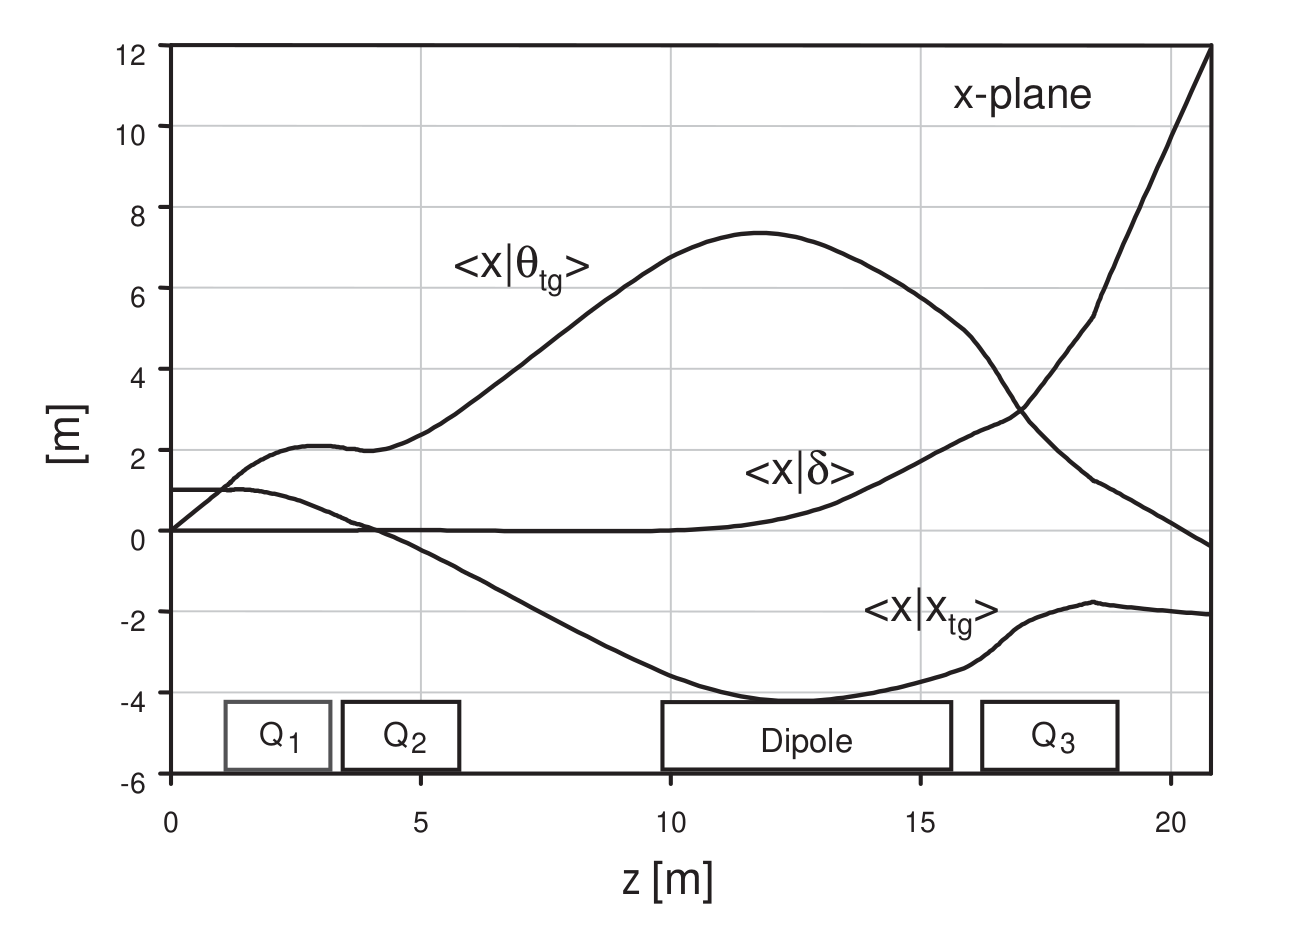
\includegraphics[width=0.50\linewidth]{hrs_transport_x}
    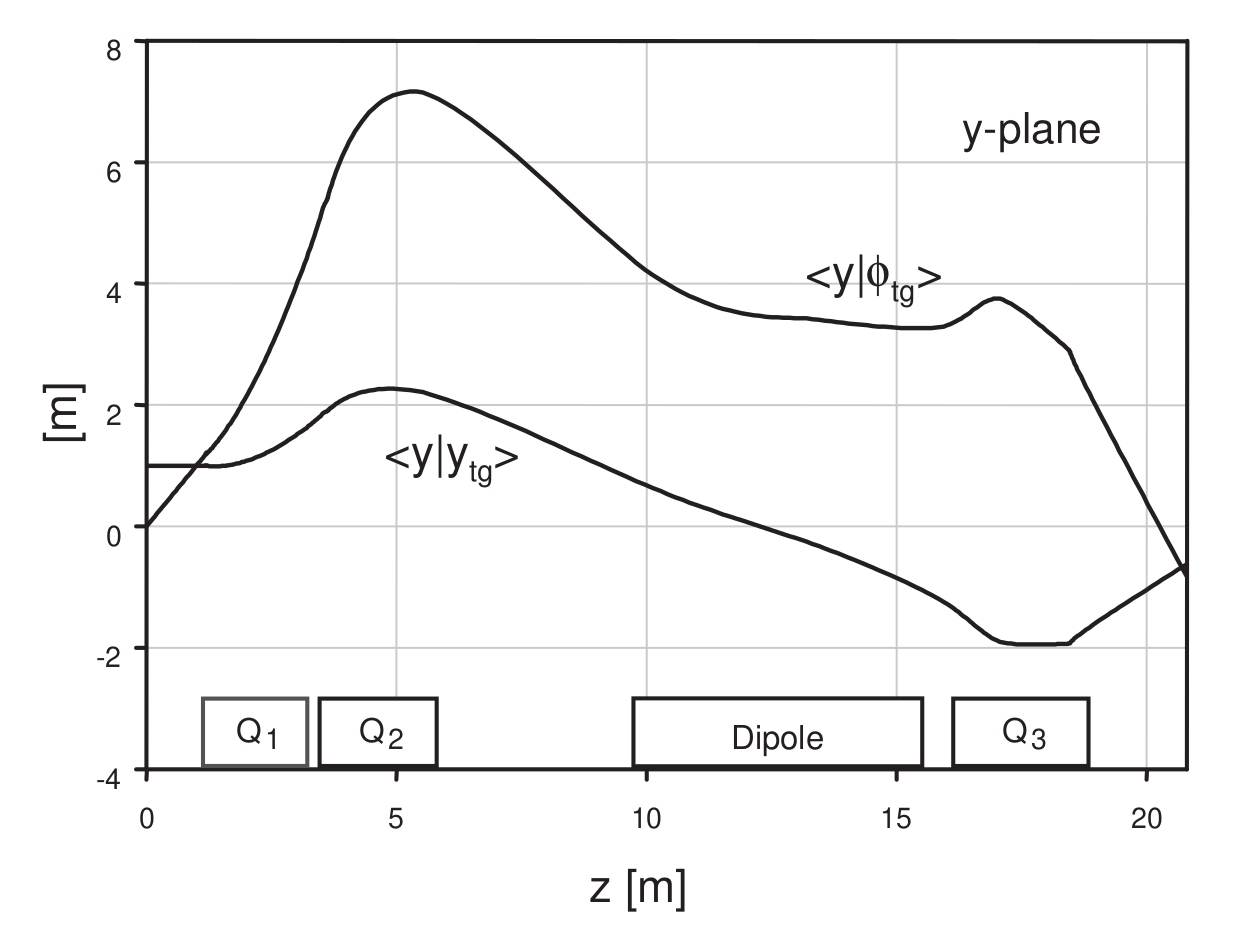
\includegraphics[width=0.48\linewidth]{hrs_transport_y}
    \caption{Transportation plot of HRS. One can clearly see the dispersion effect
    due to shift in momentum ($\delta$) in the Dipole area and the convergent effect
    of Q3.}
    \label{fig:hrs_transport}
\end{figure}

Actually, we don't need to measure every element of T, some elements are obviously
0. E.x. $\delta$ should be not be changed by any magnetic field, so $T_{5i, i\ne 5} = 0$.
The design of HRS tells us that the dispersion depends only on $\delta$, but not
on $\theta$ or $\phi$, so $x|\theta = 0$. Different planes should not
interfere with each other, so that $x|y = x|\phi = \theta|y = \theta|\phi 
= y|x = y|\theta = \phi|x = \phi|\theta = 0$. This is a sparse matrix.

The matrix elements were measured using beam trajectory with sieve slit collimator
inserted in. When the sieve slit collimator was put in, the electron trajectory
from different holes were naturally separated on the focal plane, which allowed
us to match them to sieve holes one by one. With a reasonable inital value of 
the transportation matrix (from previous experiments),
we could reconstruct electron's trajectory on the sieve plane using Eq. \ref{eq:reconstruction}.
By tuning the matrix element, the one that minizes the distance of each electron's trajectory on the sieve
plane from its corresponding hole center was identified as the transportation
matrix, so this is a linear regression problem. The identification of the septum 
and HRS current was based on the sieve pattern calculated from the 
transportation matrix. 

% The transportation matrix was extracted for following optics runs:
% \begin{table}
%     \centering
% \end{table}
% what's the difference between PREX-II and CREX?
% how many non-zero elements on the initial matrix?
% which run was used? how different runs/number of effects affect the final result
% energy on the quartz plane:

%%%%%%%%%%%%%%%%%%%%%%%%%%%%%%%%%%%%%%%%%%%%%%%%
\subsection{Scattering Angle $\theta_{lab}$}
The parameter that directly reflects the quality of simulation is the scattering
angle, while it was more convenient to use the Target Coordinate System (TCS) 
than the Hall Coordinate System (HCS) in simulation, we finally were comparing
the scattering angle in the lab frame. The 2 coordinate systems and the transportation
between them are defined below.

\begin{itemize}
    \item Hall Coordinate System: origined at the center of the hall and
	cross the beam line.  $\hat{Z}$ is along the beam line, pointing downstream; 
	$\hat{y}$ points up and $\hat{x}$ points left to form a RH coordinate system.
    \item Target Coordinate System: each HRS specific, the transport coordinate at target position.
	$\hat{z}$ is along the beam trajectory, pointing away the target, 
	$\hat{x}$ in the dispersive plane and points down, $\hat{y}$ is perpendicular
	to the dispersive plane and points away (toward) the beamline for L-HRS (R-HRS).
\end{itemize}

\begin{figure}[h!]
    \begin{subfigure}[b]{0.5\textwidth}
	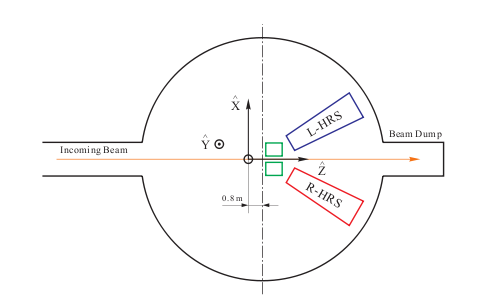
\includegraphics[width=\linewidth]{HCS}
	\caption{Top view of HCS}
    \end{subfigure}
    \begin{subfigure}[b]{0.5\textwidth}
	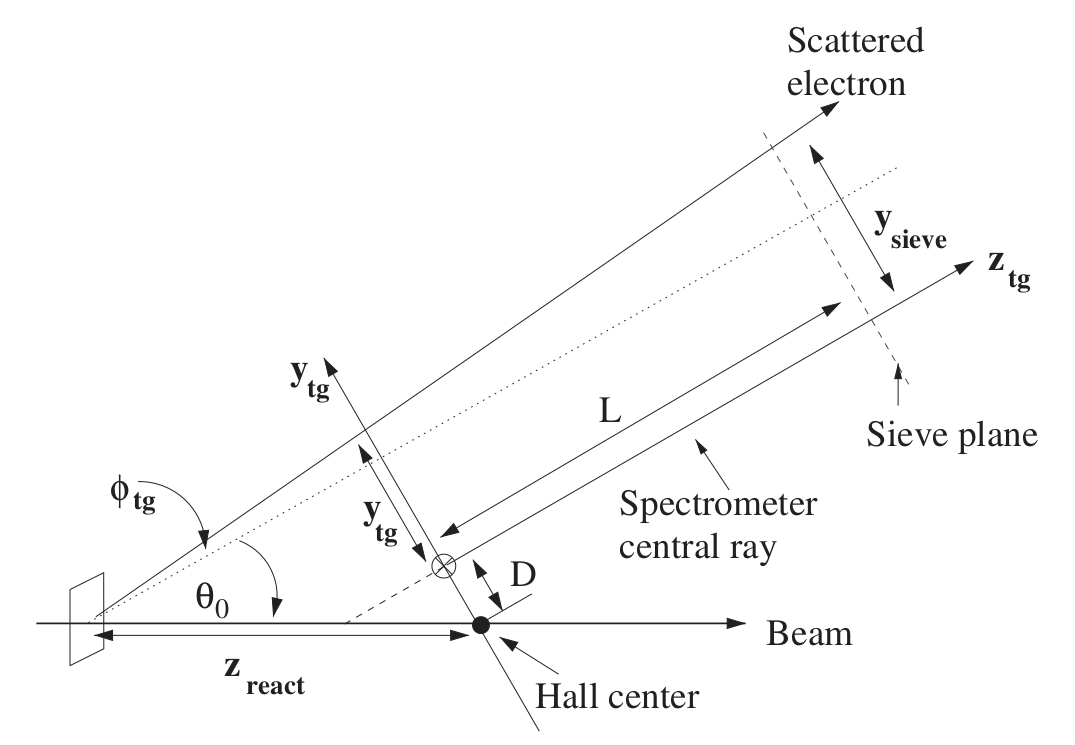
\includegraphics[width=\linewidth]{TCS}
	\caption{Top view of TCS}
    \end{subfigure}
    \caption{Schematic plot of HCS and TCS. The Hall center is the origin of the 
    HCS, but the target doesn't necessary lie in the Hall center. The distance
    from the Hall center to the sieve plane L is constant, which is used to
    identify the origin of the TCS. In ideal case, the origins of both coordinate
    systems will overlap.}
\end{figure}

The relationship between HCS and TCS is:
\begin{equation}
    \begin{pmatrix}
	x_{tg}	\\
	y_{tg}	\\
	z_{tg}	\\
    \end{pmatrix}
    =
    \begin{pmatrix}
	\cos(90^\circ)   & -\sin(90^\circ)    & 0	\\
	\sin(90^\circ)   & \cos(90^\circ)     & 0	\\
	0   & 0     & 1	\\
    \end{pmatrix}
    \begin{pmatrix}
	\cos(-\theta_0)	& 0 & -\sin(-\theta_0)  \\
	0		& 1 & 0		\\
	\sin(-\theta_0)	& 0 & \cos(-\theta_0)  \\
    \end{pmatrix}
    \begin{pmatrix}
	x   \\
	y   \\
	z   \\
    \end{pmatrix}
\end{equation}

\begin{equation}
    \left.
    \begin{aligned}
	x_{tg}	&= -y	\\
	y_{tg}	&= x\cos\theta_0 + z\sin\theta_0    \\
	z_{tg}	&= -x\sin\theta_0 + z\cos\theta_0   \\
    \end{aligned}
    \right\}
    \iff
    \left\{
    \begin{aligned}
	x   &= y_{tg}\cos\theta_0 + z_{tg}\sin\theta_0	\\
	y   &= -x_{tg}	\\
	z   &= -y_{tg}\sin\theta_0 + z_{tg}\cos\theta_0   \\
    \end{aligned}
    \right.
\end{equation}
Define $R = \left(x^2 + y^2 + z^2\right)^{1/2} = z_{tg} \left(\phi^2_{tg} + \theta^2_{tg} + 1\right)^{1/2}$.
So the scattering angle in the lab frame will be:
\begin{equation}
    \cos\theta = \frac{z}{R} = \frac{-\phi_{tg}\sin\theta_0 + \cos\theta_0}{\left(\phi^2_{tg} + \theta^2_{tg} + 1\right)^{1/2}}
\end{equation}
For data, $\theta_0$ was identified to be $4.789^\circ$ ($4.771^\circ$) for
L-HRS (R-HRS). In simulation, both arms used $4.74^\circ$. Note that $\theta_{lab}$
is a post-target (apparent) quantity, which includes effect of post-vertex radiation and
multi-scattering, not the `real' scattering angle (vertex quantity) at the vertex 
where the interesting PV elastic scattering happens. The correction from the apparent 
distribution to the vertex distribution is about 1.5\%.
\begin{figure}[h!]
    \centering
    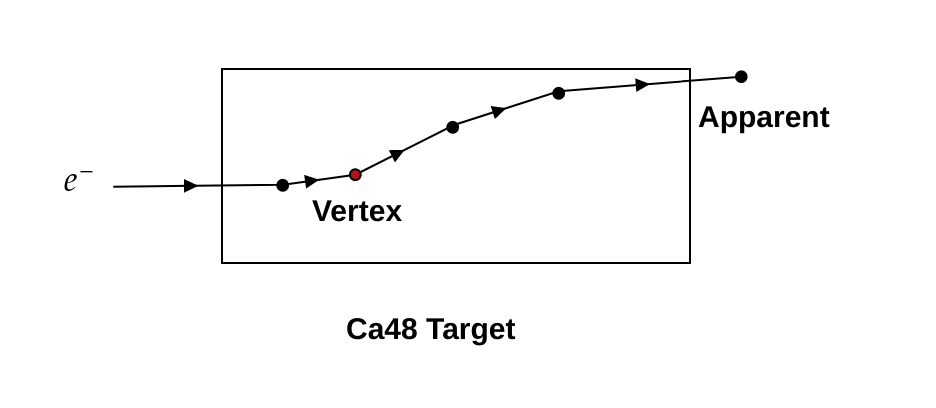
\includegraphics[width=0.5\linewidth]{scattering}
    \caption{Schematic plot of vertex and apparent quantities.}
\end{figure}

%%%%%%%%%%%%%%%%%%%%%%%%%%%%%%%%%%%%%%%%%%%%%%%%
\subsection{Data}
\begin{table}[h!]
    \begin{tabular}{c c | c | c | c c c c}
	\hline
	Exp & Arm   & Dipole p0 ($GeV$)    & Septum ($A$)  & Q1 ($A$)	& A2 ($A$) & Q3 ($A$)  \\
	\hline
	\multirow{2}{*}{PREX-II} & Left	& 0.95285   & 333   & 118.50	& 407.70    & 450.76    \\
				 & Right& 0.95284   & 333   & 118.55	& 404.07    & 446.90    \\
	\hline
	\multirow{2}{*}{CREX}	& Left	& 2.183522  & 801   & 225.387	& 934.273   & 981.301    \\
				& Right	& 2.183499  & 801   & 230.916	& 925.955   & 981.301    \\
	\hline
    \end{tabular}
    \caption{PREX-II and CREX tune}
    \label{tab:pcrex_tune}
\end{table}

To determine the new tune of septum and HRS settings for CREX, we started with 
PREX-II tune, scaled it to CREX momentum. To know the appropriate septum 
current that will bridge the central ray into HRS axis we tuned septum and 
Q1 current in 2 steps: coarse and fine tuning. During coarse tuning, we
changed septum and Q1 current by a large step: 10\% (\textbf{central ray search});
and then fine tuned the septum current in a smaller step: 2.5\% to find out
the largest acceptance (\textbf{inner edge search}).

During the central ray search, if the septum current was inappropriate, 
then when we changed the Q1 current, the central hole in reconstructed sieve 
pattern plot would shift, as shown in Fig. \ref{fig:central_ray_0}.
\begin{figure}[h!]
    \centering
    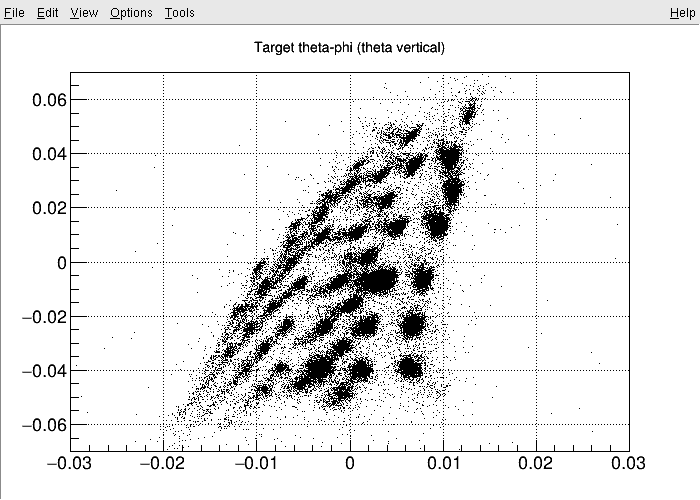
\includegraphics[width=0.32\linewidth]{minus10_septum_minus10_Q1_right}
    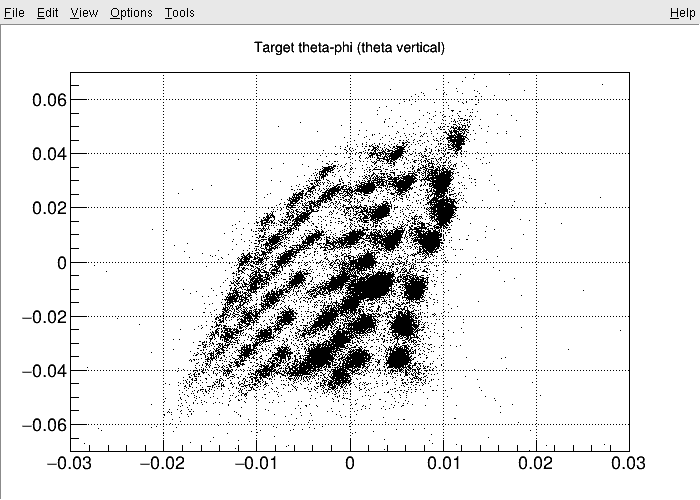
\includegraphics[width=0.32\linewidth]{minus10_septum_nominal_Q1_right}
    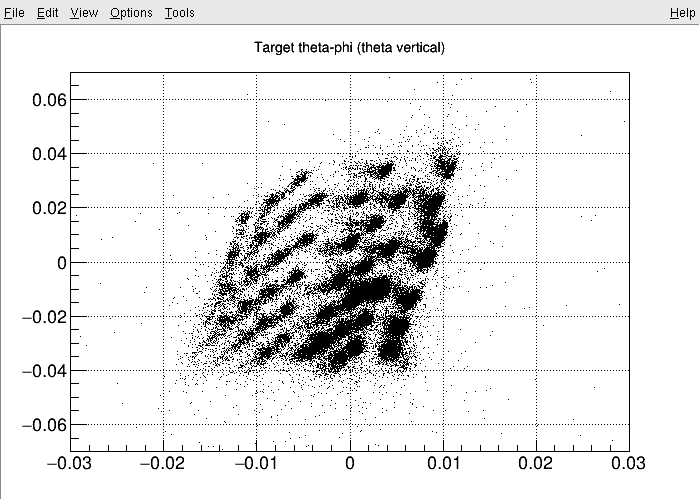
\includegraphics[width=0.32\linewidth]{minus10_septum_plus10_Q1_right}
    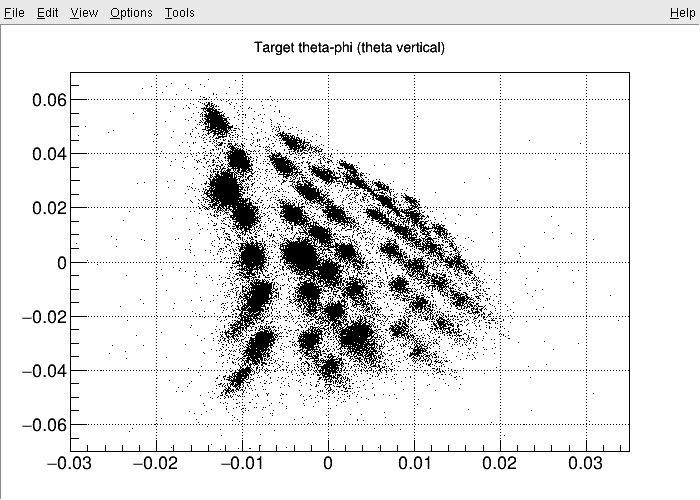
\includegraphics[width=0.32\linewidth]{minus10_septum_minus10_Q1_left}
    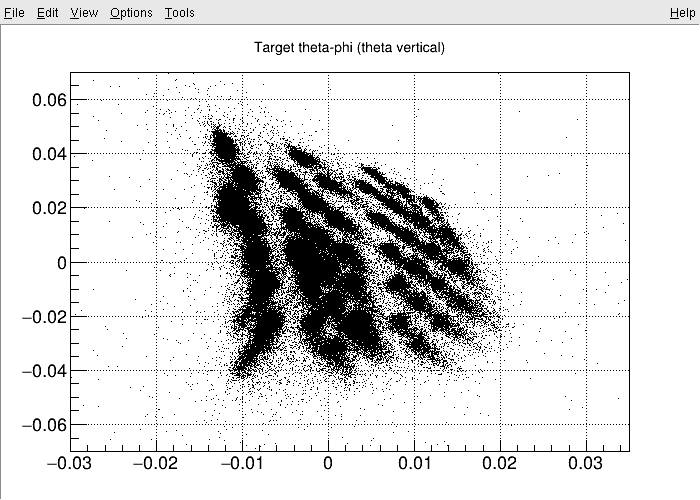
\includegraphics[width=0.32\linewidth]{minus10_septum_nominal_Q1_left}
    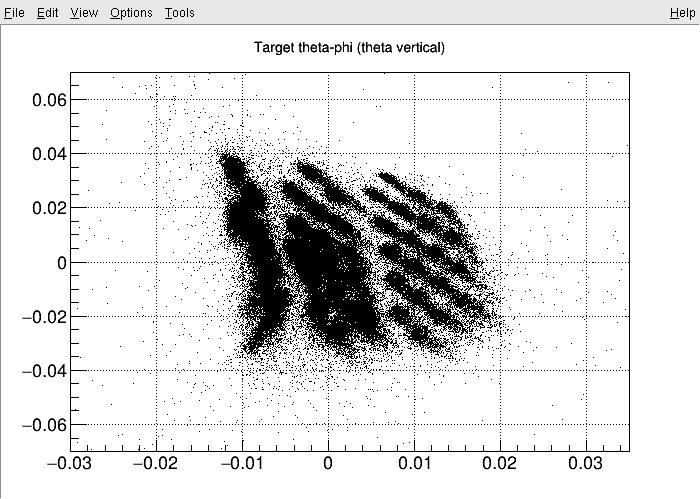
\includegraphics[width=0.32\linewidth]{minus10_septum_plus10_Q1_left}
    \caption{Sieve pattern plots for -10\% septum current
    and varied Q1 current, from left to right: -10\%, nominal and +10\% Q1 current.
    With different Q1 current, the sieve pattern twist, and the central hole 
    shifts in $\theta$, so the septum current is not a good value.}
    \label{fig:central_ray_0}
\end{figure}

\begin{figure}[h!]
    \centering
    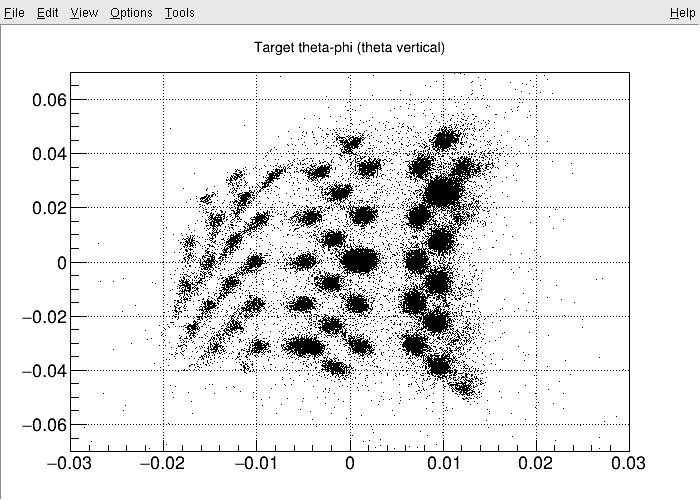
\includegraphics[width=0.32\linewidth]{nominal_septum_minus10_Q1_right}
    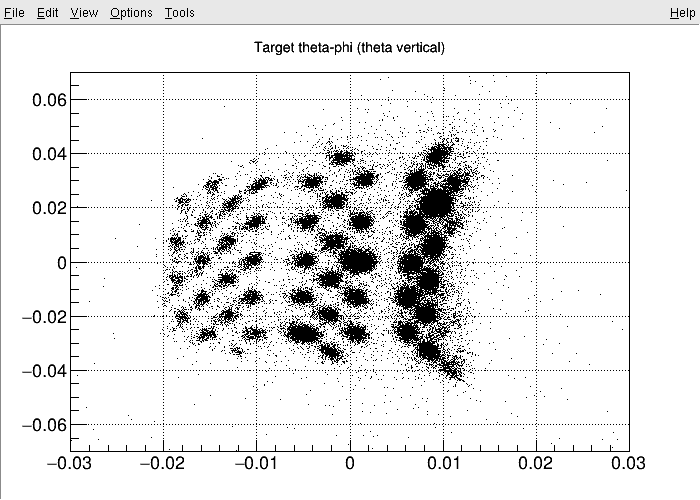
\includegraphics[width=0.32\linewidth]{nominal_septum_nominal_Q1_right}
    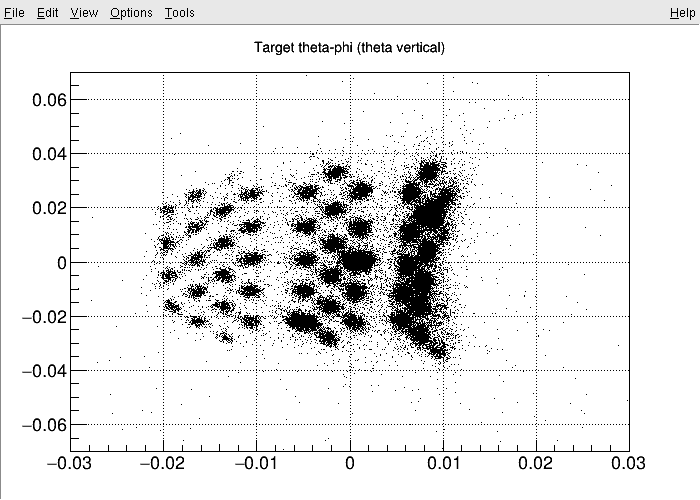
\includegraphics[width=0.32\linewidth]{nominal_septum_plus10_Q1_right}
    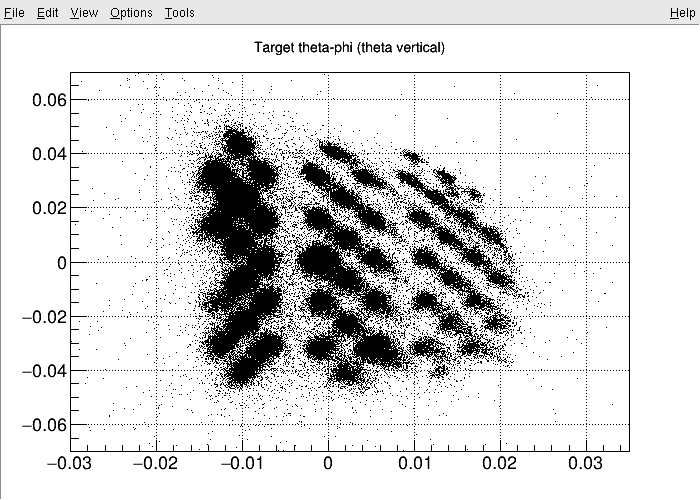
\includegraphics[width=0.32\linewidth]{nominal_septum_minus10_Q1_left}
    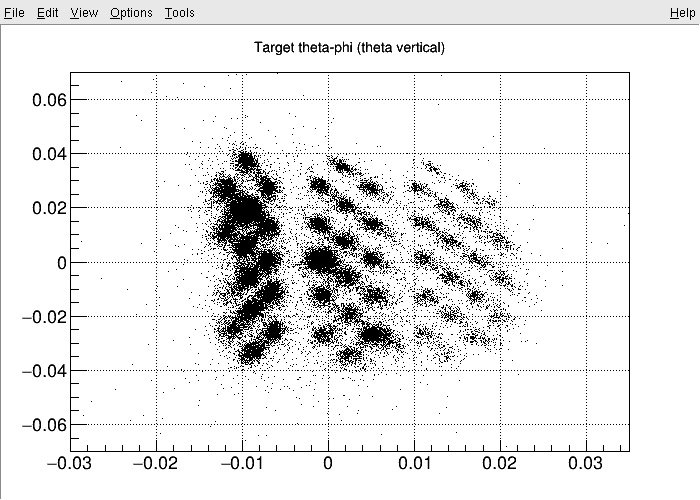
\includegraphics[width=0.32\linewidth]{nominal_septum_nominal_Q1_left}
    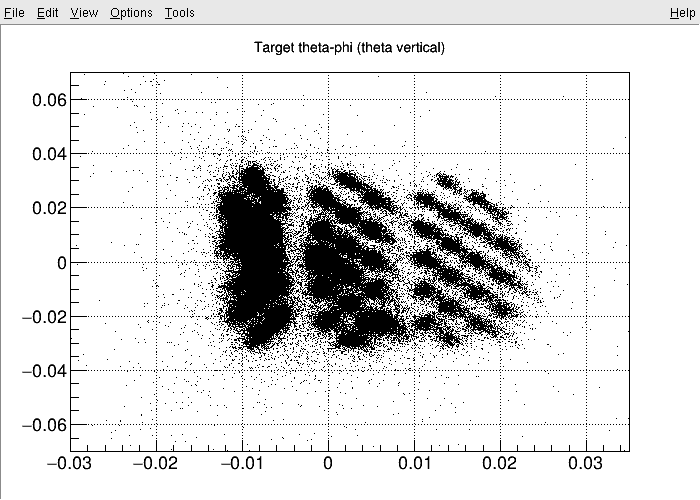
\includegraphics[width=0.32\linewidth]{nominal_septum_plus10_Q1_left}
    \caption{Sieve pattern plots for nominal (scaled from PREX-II setting) septum current
    and varied Q1 current, from left to right: -10\%, nominal and +10\% Q1 current.
    Top row is right arm and bottom row is left arm. With different Q1 current,
    the sieve pattern twist, but the central hole keeps at the same position, 
    which means the central ray goes through the axis of the HRS.}
    \label{fig:central_ray_1}
\end{figure}

Fig. \ref{fig:central_ray_1} told us the nominal septum current and HRS settings was not a bad choice,
so we could move on to inner edge search with this septum nominal value: to
see more inner holes -- holes with largest (smallest) phi in Left (right) arm.
It turned out a 5\% increasement from the nominal value gave us the largest 
acceptance, which corresponds to a septum current of: $1.05 \times (333*2.183522/0.95285) = 801.25 \ A$.
\begin{figure}[h!]
% https://logbooks.jlab.org/entry/3748464
    \begin{tikzpicture}
	\begin{scope}
	    \node[anchor=south west, inner sep=0] (image) at (0, 0)
	    {	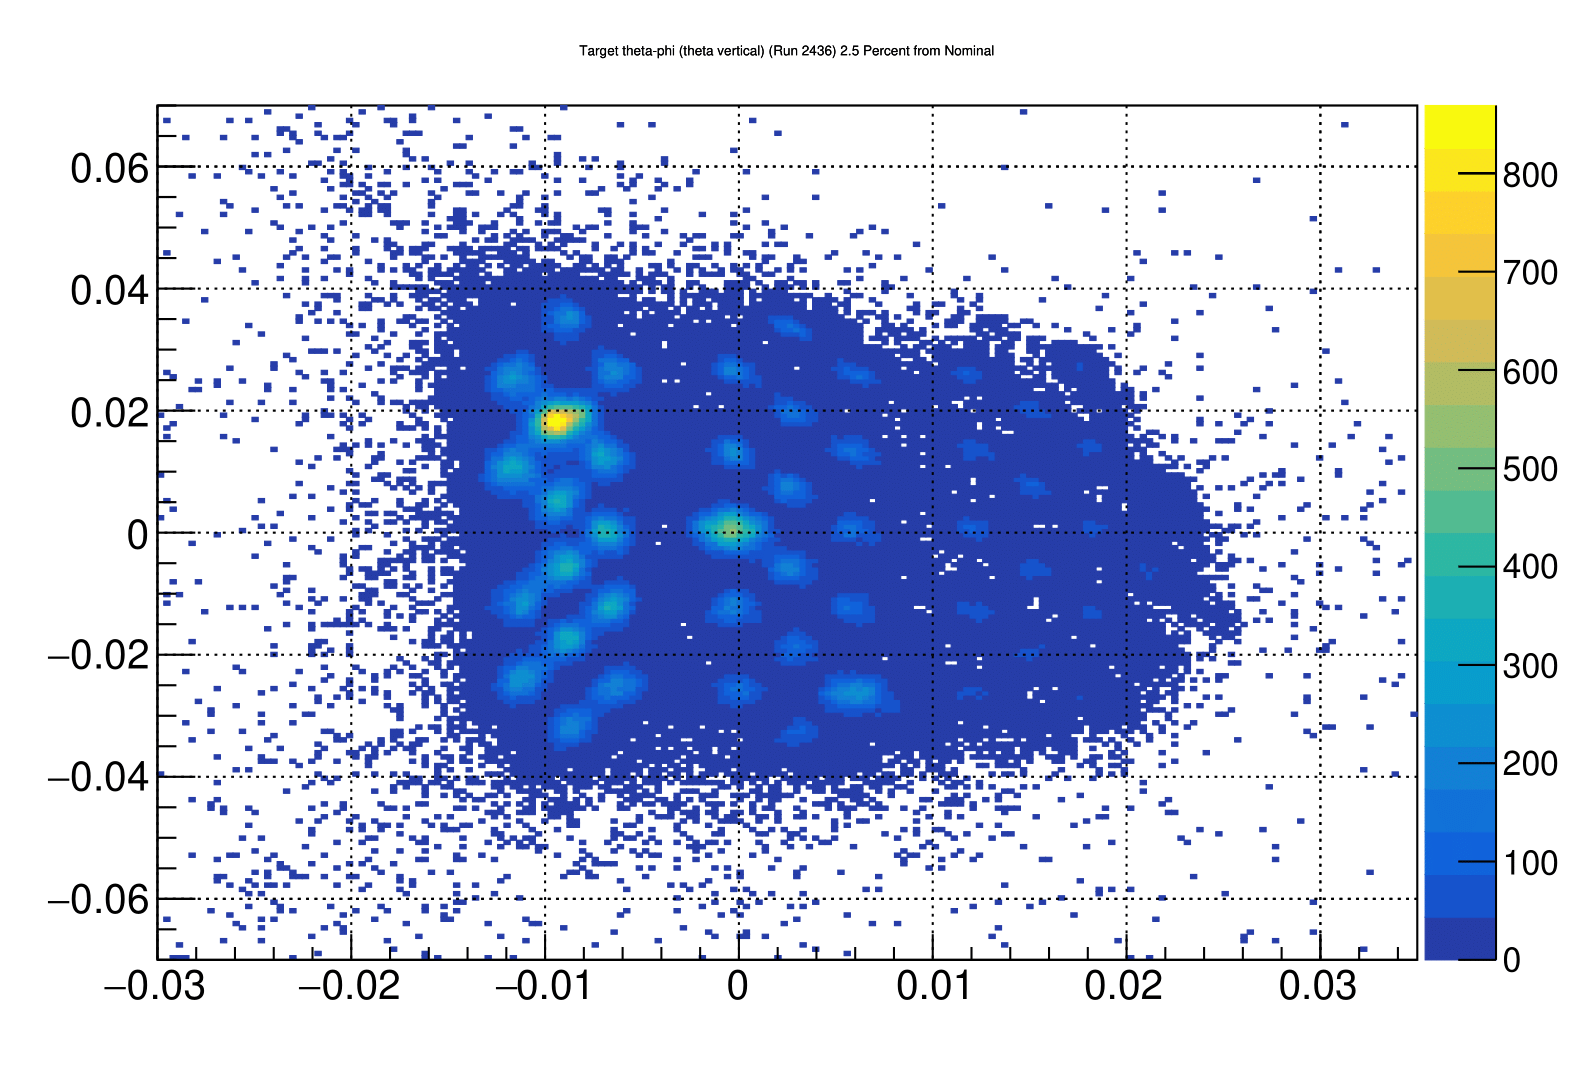
\includegraphics[width=0.49\linewidth]{plus2.5_septum} 
		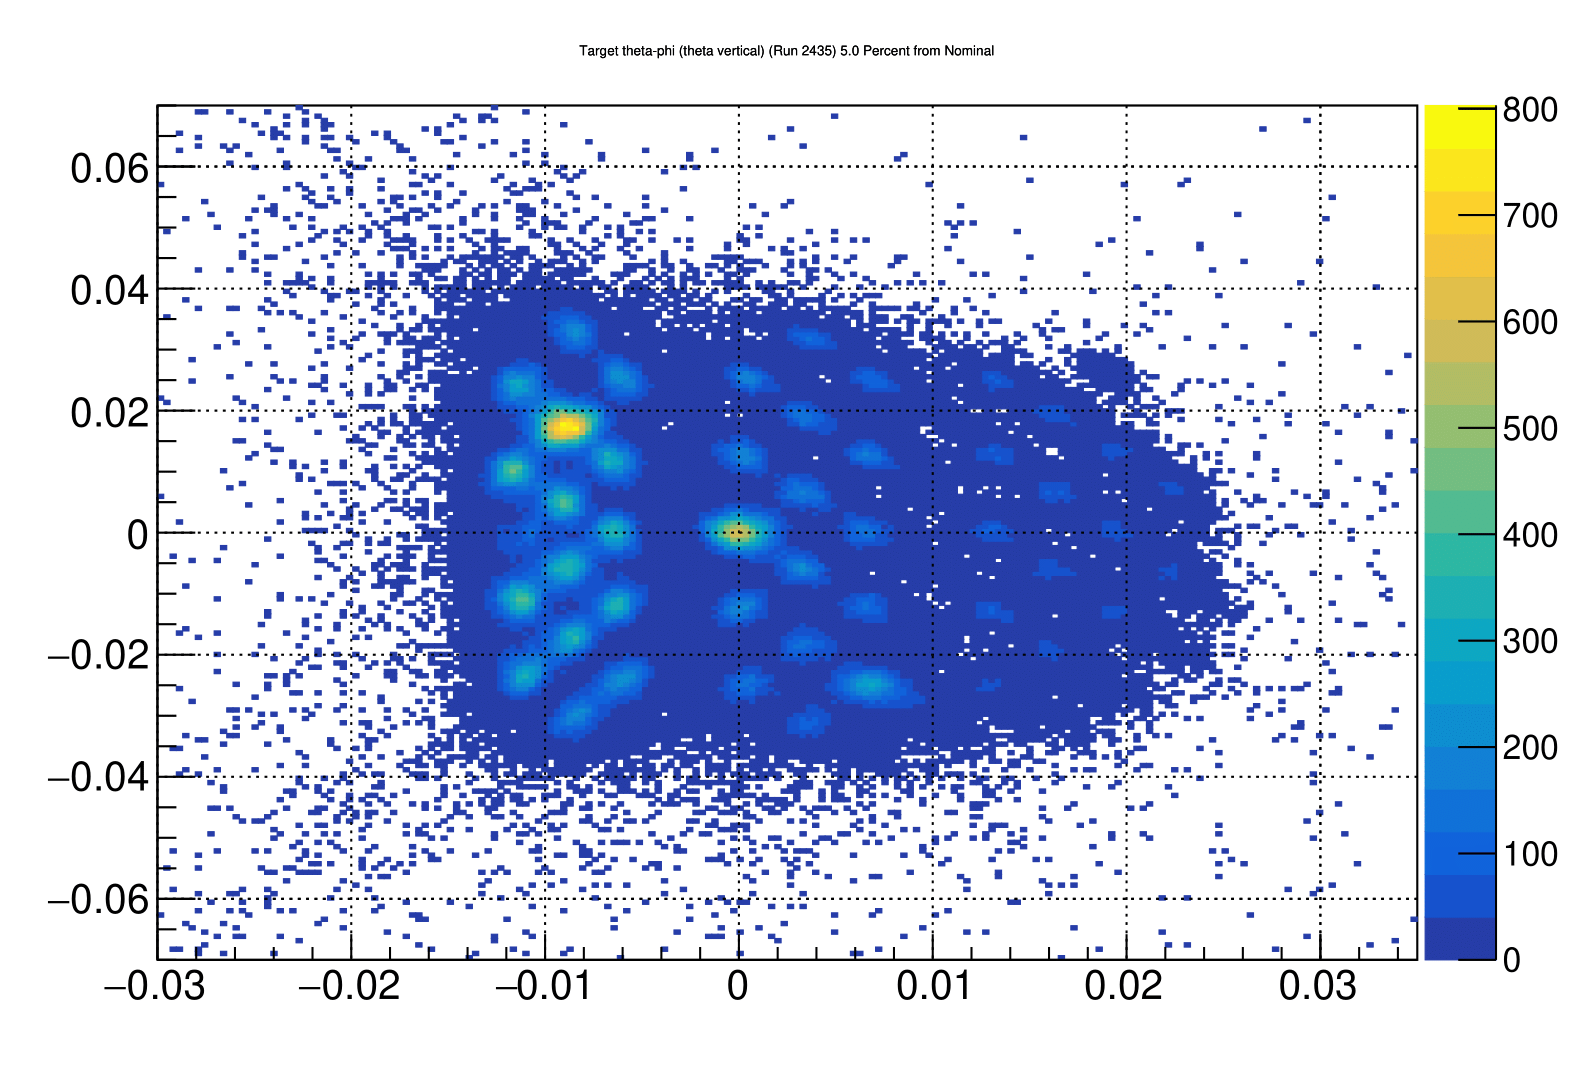
\includegraphics[width=0.49\linewidth]{plus5_septum} 
	    };
	    \begin{scope}[x={(image.south east)}, y={(image.north west)}]
		\draw [thick, Red] (0.67, 0.5) circle (4 pt);
		\draw [thick, Yellow] (0.874, 0.46) circle (4 pt);
		\draw [thick, Yellow] (0.874, 0.55) circle (4 pt);
	    \end{scope}
	\end{scope}
    \end{tikzpicture}
    \begin{tikzpicture}
	\begin{scope}
	    \node[anchor=south west, inner sep=0] (image) at (0, 0)
	    {	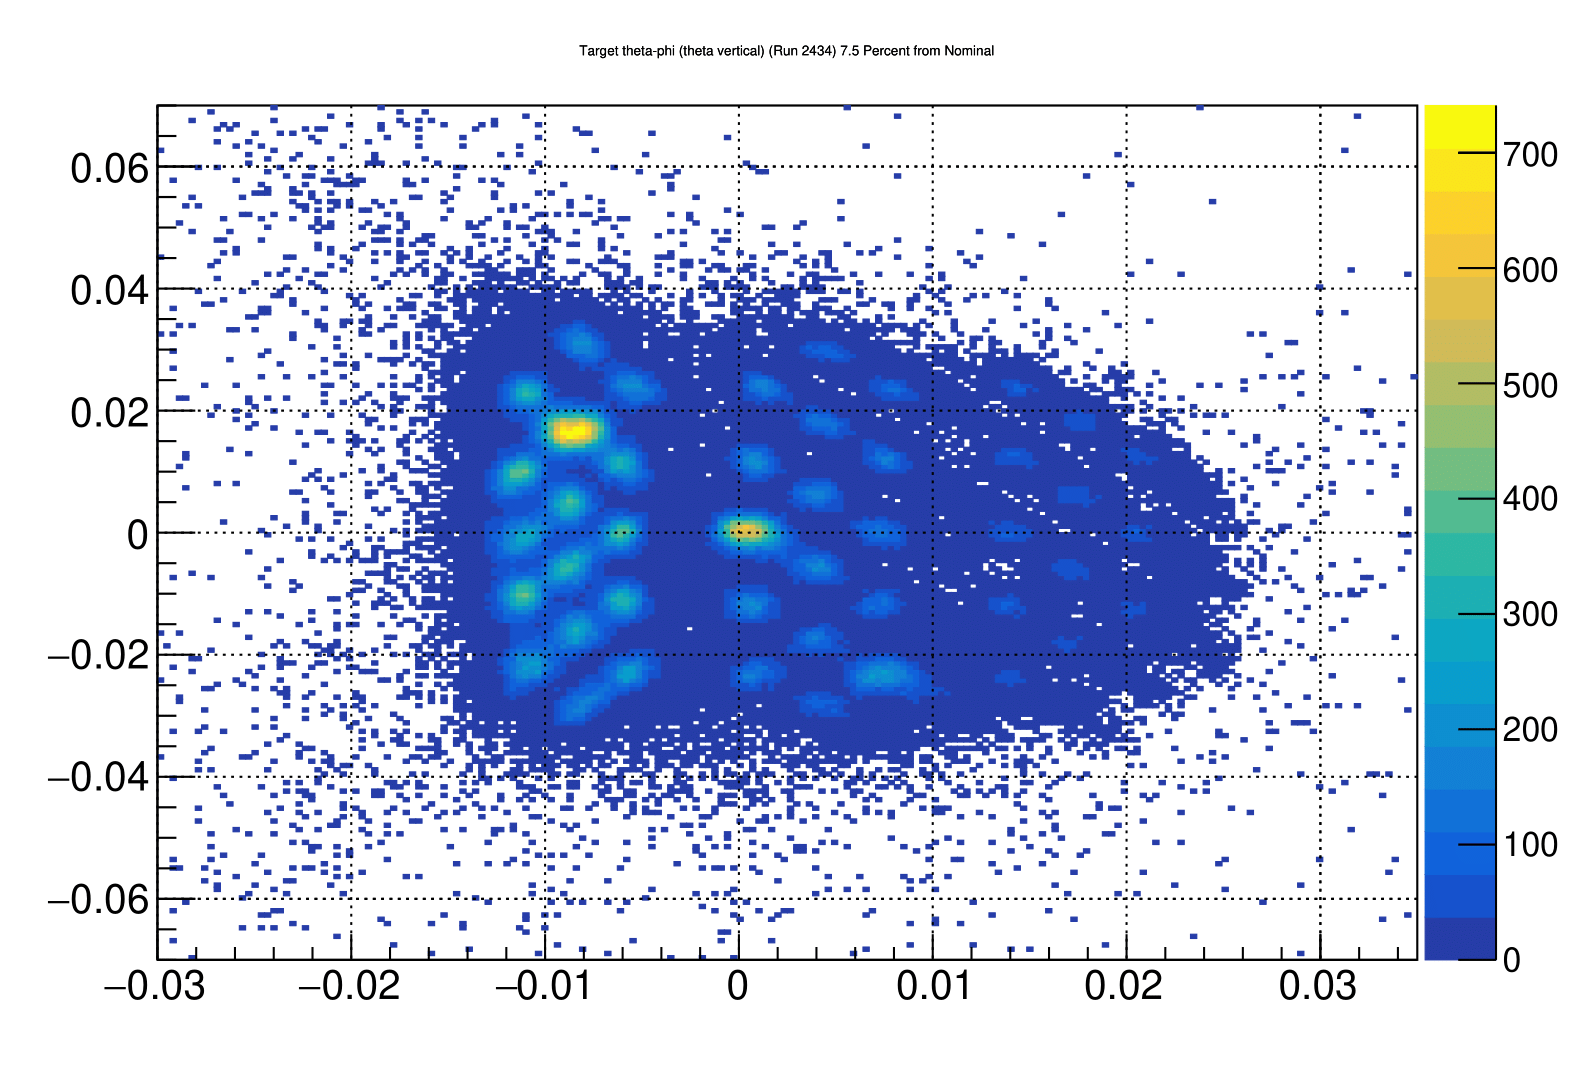
\includegraphics[width=0.49\linewidth]{plus7.5_septum} 
		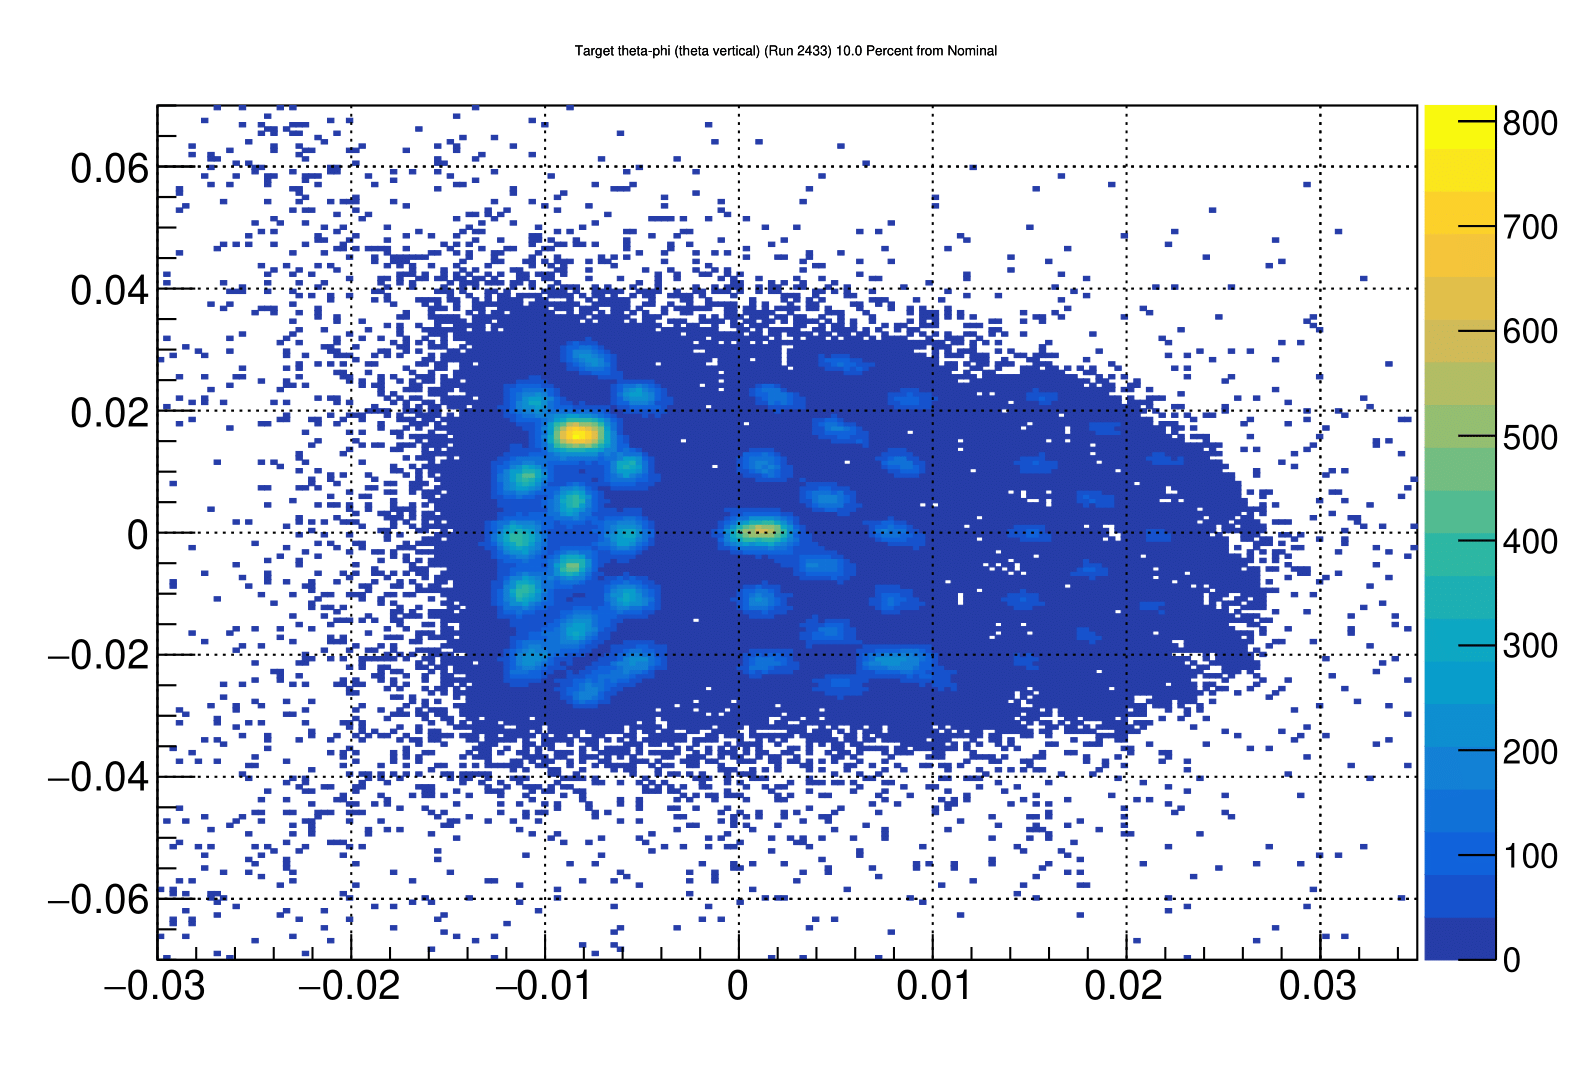
\includegraphics[width=0.49\linewidth]{plus10_septum} 
	    };
	\end{scope}
    \end{tikzpicture}
    \caption{Inner edge search on the left arm. Septum current from top left
    to bottom right: +2.5\%, +5\%, +7.5\%, +10\%. The inner middle hole starts
    to appear since +5\%, and outer holes disappear since 7.5\%, so the best
    septum current was chosed to be +5\%}
\end{figure}

With selected septum current, we continued to minimize beam spot size on the detector
plane, a fine tune of Q1 and Q3 gave us the smallest detector spot size with
Q1 -17\% (-15\%) from the nominal value on left (right) arm, and Q3 -5\% from
the nominal value on both arms, which led to the final CREX tune as shown in
Table \ref{tab:pcrex_tune}.
\begin{table}[h!]
    \begin{tabular}{c c | c c c | c c c}
	\hline
	& & \multicolumn{3}{c}{Left} & \multicolumn{3}{c}{Right}  \\
	\hline
	Q1(\%)  & Q3 (\%)    & run   & $\sigma_y\ (cm)$  & $\sigma_x\ (cm)$   & run   & $\sigma_y\ (cm)$    & $\sigma_x\ (cm)$    \\
	\hline
	0   & 0	    & 2524  & 0.9604	& 1.634	    & 21604	& 0.009564  & 0.01503 \\
	-5  & 0	    & 2525  & 0.955	& 1.188	    & \multicolumn{3}{c}{Left arm only}    \\
	-10 & 0	    & 2526  & 1.005	& 0.9063    & \multicolumn{3}{c}{Left arm only}    \\ 
	-15 & 0	    & 2527  & 0.1078	& 0.7314    & \multicolumn{3}{c}{Left arm only}    \\ 
	-20 & 0	    & 2528  & 1.182	& 0.6801    & \multicolumn{3}{c}{Left arm only}    \\ 
	\hline                              
	-11 & 0	    & 2529  & 1.012	& 0.8767    & 21609	& 0.009315  & 0.007337	\\
	-12 & 0	    & 2530  & 1.012	& 0.8349    & 21610	& 0.009429  & 0.006957  \\
	-13 & 0	    & 2531  & 1.033	& 0.7835    & 21611	& 0.009526  & 0.006682  \\
	-14 & 0	    & 2532  & 1.057	& 0.7515    & 21612	& 0.009623  & 0.06367   \\
	\hline                              
	-13 & +10   & 2533  & 1.754	& 1.929	    & 21613	& 0.0162    & 0.0215    \\
	-13 & +5    & 2534  & 1.374	& 0.7282    & 21614	& 0.01276   & 0.01174   \\
	-13 & -5    & 2535  & 0.8357	& 0.9751    & 21615	& 0.008422  & 0.008514  \\
	-13 & -10   & 2536  & 0.8855	& 1.482	    & 21616	& 0.008891  & 0.01387   \\
	\hline
	% -13 & -15   & 2537  & 1.133	& 2.042	    & 21617	& 1.141   & 2.051   \\
	-13 & -2    & 2538  & 0.9415	& 0.8761    & 21618	& 0.9117    & 0.7078  \\
	-13 & -4    & 2539  & 0.8602	& 0.9181    & 21619	& 0.8493    & 0.7912  \\
	-13 & -7    & 2540  & 0.8182	& 1.154	    & 21620	& 0.8304    & 1.027   \\
	-13 & -9    & 2541  & 0.8445	& 1.389	    & 21621	& 0.8545    & 1.268   \\
	-15 & -5    & 2542  & 0.8354	& 0.8869    & 21622	& 0.827	    & 0.7563  \\
	\hline
	-15 (R);-17 (L)	& -5	&2543	& 0.8409	& 0.8315  & 21623 & 0.8382	& 0.7615  \\
	\hline
    \end{tabular}
    \caption{Beam spot size with different HRS settings.}
\end{table}

%%%%%%%%%%%%%%%%%%%%%%%%%%%%%%%%%%%%%%%%%%%%%%%%
\subsection{Simulation}
The simulation was not exactly the reproduction of reality. We used GEANT4 to
simulate the geometry of each component based on the designed values, the
septum magnetic field was scaled from a field map file sampled from the septum
at $j_0 = -1320\ A/cm^2$: % FIXME why?
% https://prex.jlab.org/DocDB/0001/000160/001/g4hrs_tune.pdf
\begin{equation}
    B'_{xyz} = \frac{J}{J_0} \times \frac{P}{P_0} \times B_{xyz}
\end{equation}
The same for HRS field: % how to know HRS field at each position
\begin{equation}
    B'_{i = Q1, Q2, D, Q3} = \frac{P}{P_0} \times B_i
\end{equation}

Using this construction, we could firstly vary the septum current to choose the
one that most matched the data, then scaned through collimator shift and pinch point
shift to select the best model.

\begin{figure}[h!]
    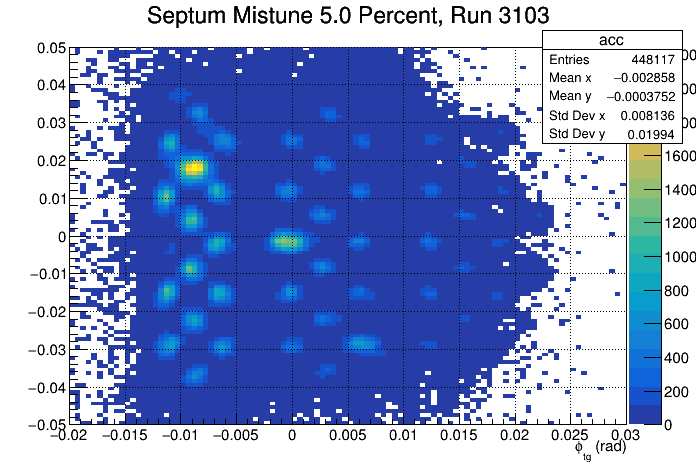
\includegraphics[width=0.49\linewidth]{sieve_run3103}
    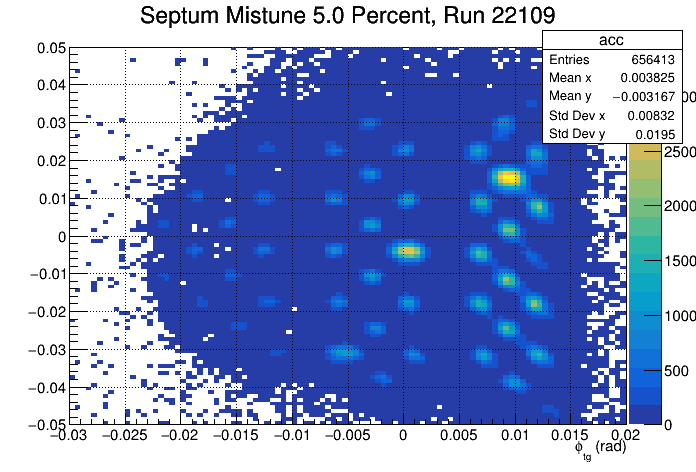
\includegraphics[width=0.49\linewidth]{sieve_run22109}
    \caption{Sieve plot of CREX tune. Centered at (-0.3, -1.5), the new beam 
    position for the new target.}
\end{figure}

Somewhat expected, a coarse scan through the septum told us the septum range
for best model: around 0-5\% above the nominal value.
\begin{figure}[h!]
    \begin{tikzpicture}
	\begin{scope}
	    \node[anchor=south west, inner sep=0] (image) at (0, 0)
	    {	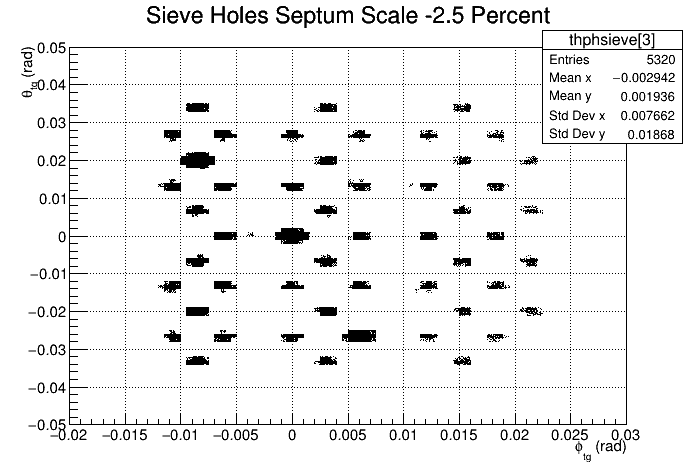
\includegraphics[width=0.49\linewidth]{sieve_sim_minus2.5_left} 
		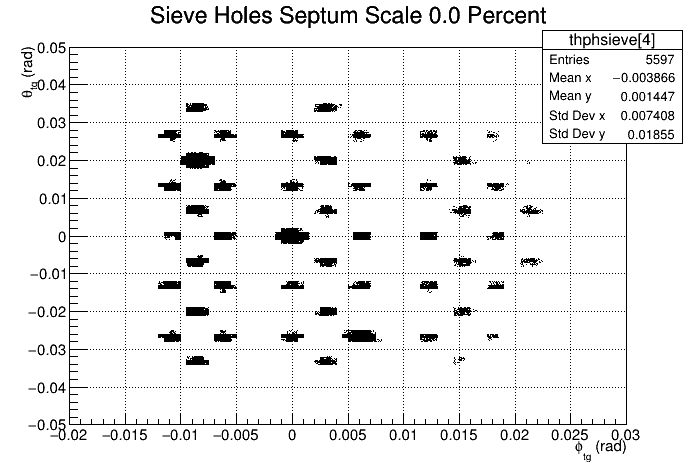
\includegraphics[width=0.49\linewidth]{sieve_sim_nominal_left} 
	    };
	\end{scope}
	\begin{scope}[x={(image.south east)}, y={(image.north west)}]
	    \draw [thick, Red] (0.12, 0.5) circle (4 pt);
	    \draw [thick, Red] (0.33, 0.78) circle (4 pt);
	    \draw [thick, Red] (0.33, 0.23) circle (4 pt);
	    \draw [thick, Red] (0.353, 0.715) circle (4 pt);
	    \draw [thick, Red] (0.353, 0.28) circle (4 pt);
	    \draw [thick, Red] (0.378, 0.655) circle (4 pt);
	    \draw [thick, Red] (0.378, 0.336) circle (4 pt);

	    \draw [thick, Red] (0.83, 0.232) circle (4 pt);
	    \draw [thick, Red] (0.855, 0.715) circle (4 pt);
	    \draw [thick, Red] (0.855, 0.282) circle (4 pt);
	\end{scope}
    \end{tikzpicture}
    \begin{tikzpicture}
	\begin{scope}
	    \node[anchor=south west, inner sep=0] (image) at (0, 0)
	    {	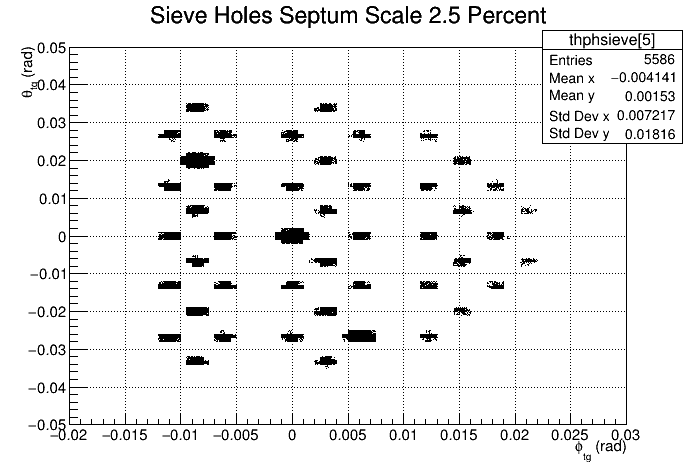
\includegraphics[width=0.49\linewidth]{sieve_sim_plus2.5_left} 
		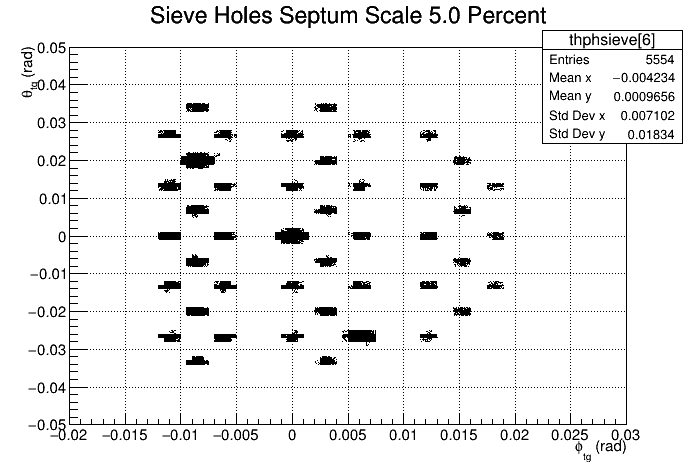
\includegraphics[width=0.49\linewidth]{sieve_sim_plus5_left} 
	    };
	\end{scope}
	\begin{scope}[x={(image.south east)}, y={(image.north west)}]
	    \draw [thick, Red] (0.88, 0.45) circle (4 pt);
	    \draw [thick, Red] (0.88, 0.55) circle (4 pt);
	\end{scope}
    \end{tikzpicture}
    \caption{Sieve pattern plots from simulation with different septum current.}
\end{figure}

\begin{figure}[h!]
    \centering
    \begin{tikzpicture}
	\begin{scope}
	    \node[anchor=south west, inner sep=0] (image) at (0, 0)
	    {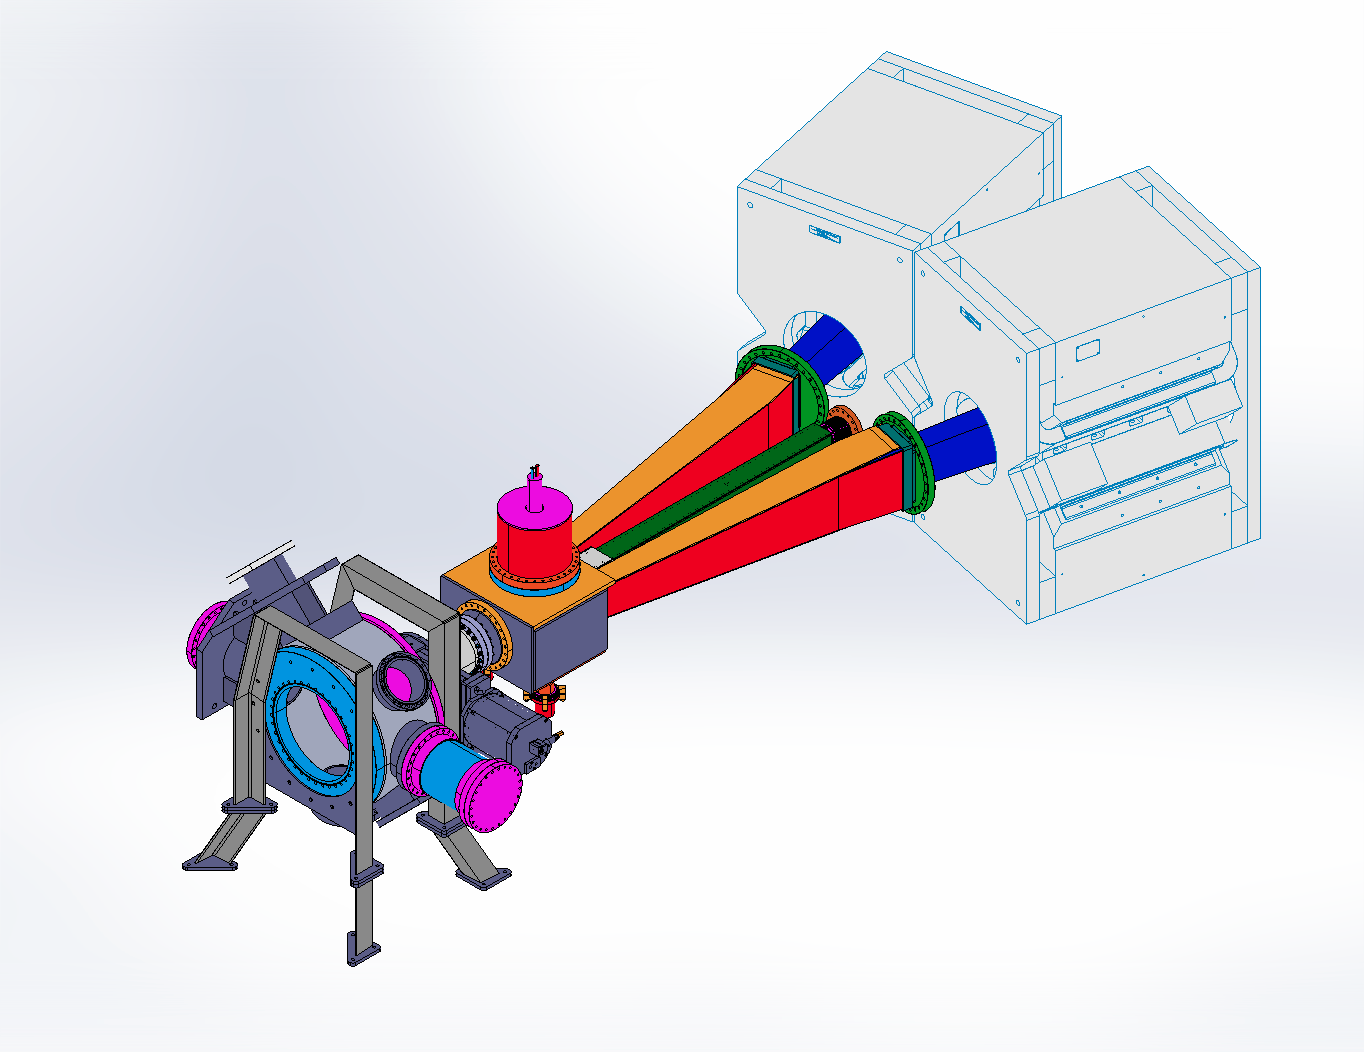
\includegraphics[width=0.5\linewidth]{pivot_region_0}};
	    \begin{scope}[x={(image.south east)},y={(image.north west)}]
		\draw[red,ultra thick] (0.44,0.44) circle (0.17 cm);
		\draw [-latex, thick, red] (0.46, 0.1) node {\scriptsize{Pinch Point}} -- (0.44,0.39);
		\node[green] (coll) at (0.7, 0.2) {\scriptsize{Collimator}};
		\draw [-latex, thick, green] (coll.north) -- (0.67,0.51);
	    \end{scope}
	\end{scope}
    \end{tikzpicture}
    \caption{Position of the pinch point and the Q1 collimator.}
\end{figure}
Then we can scan throught the pinch point and collimator shift with a fine tune
of the septum current (from -1\% to +5\%). The pinch point is the connection point
between the septum beampipe and the collimator box, whose misalignment will affect
the acceptance; another parameter we can tune is the collimator (TCS) y position,
which of course has a large impact on the acceptance. For each simulation, we
will compare the average scattering angle $\theta_{lab}$, $Q^2$ and asymmetry to
that of optics data.

\begin{figure}[h!]
    \centering
    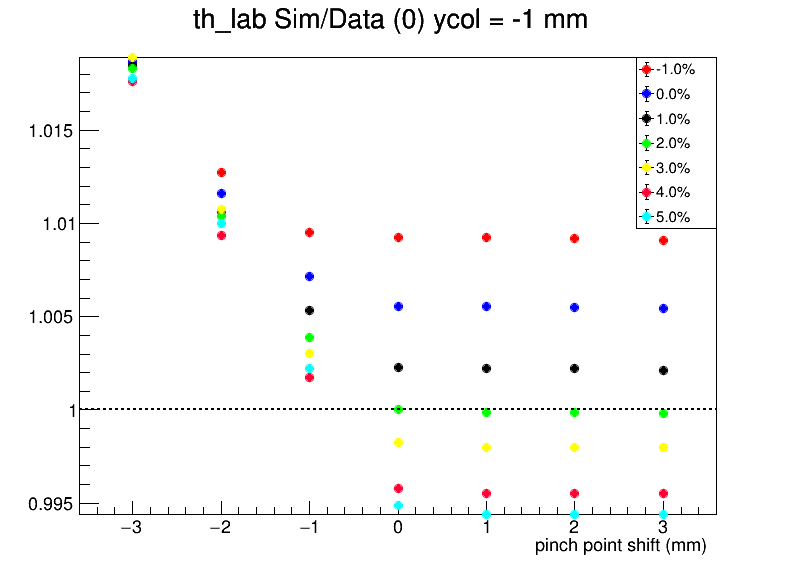
\includegraphics[width=0.32\linewidth]{pinch_scan_th_lab_-1_run0}
    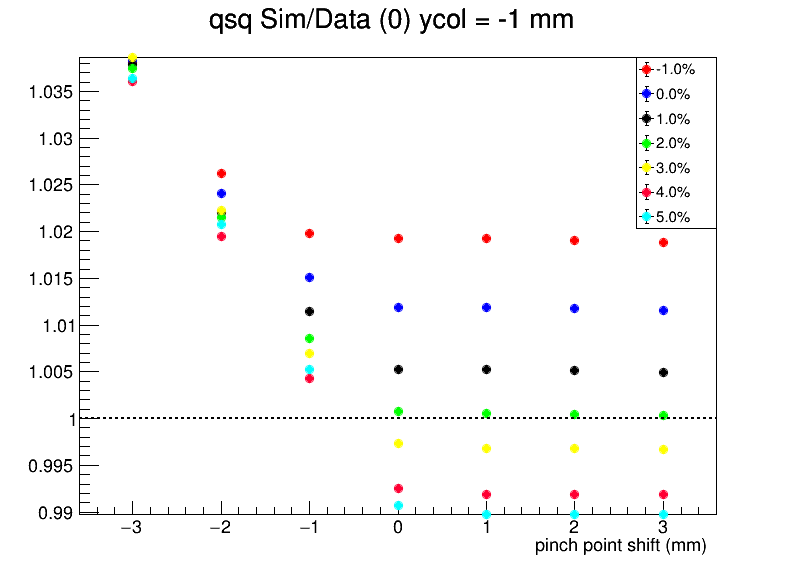
\includegraphics[width=0.32\linewidth]{pinch_scan_qsq_-1_run0}
    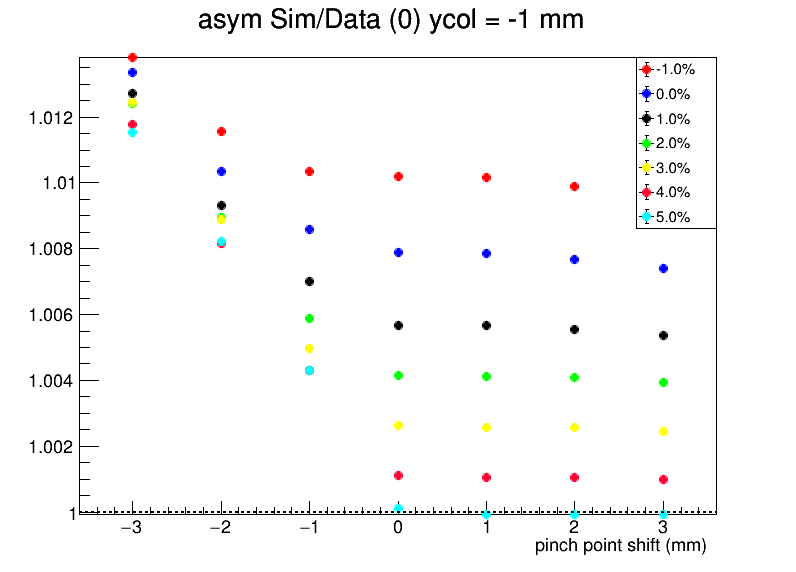
\includegraphics[width=0.32\linewidth]{pinch_scan_asym_-1_run0}
    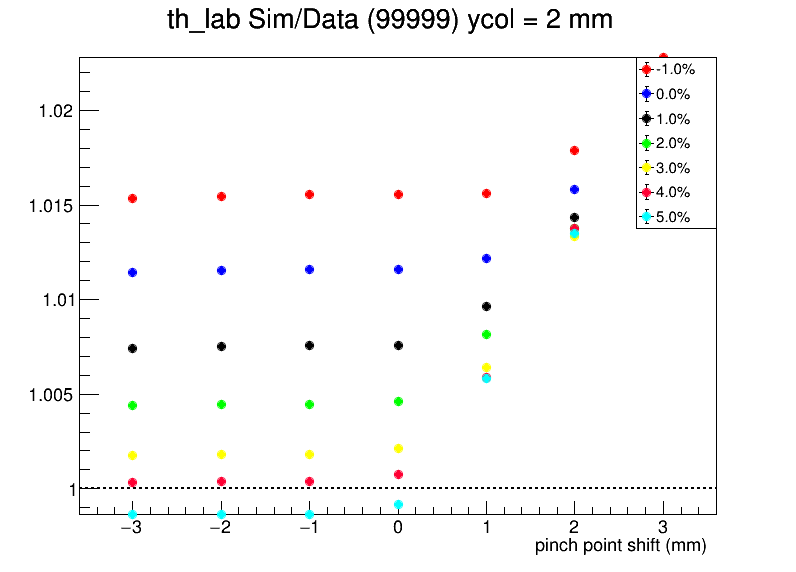
\includegraphics[width=0.32\linewidth]{pinch_scan_th_lab_2_run99999}
    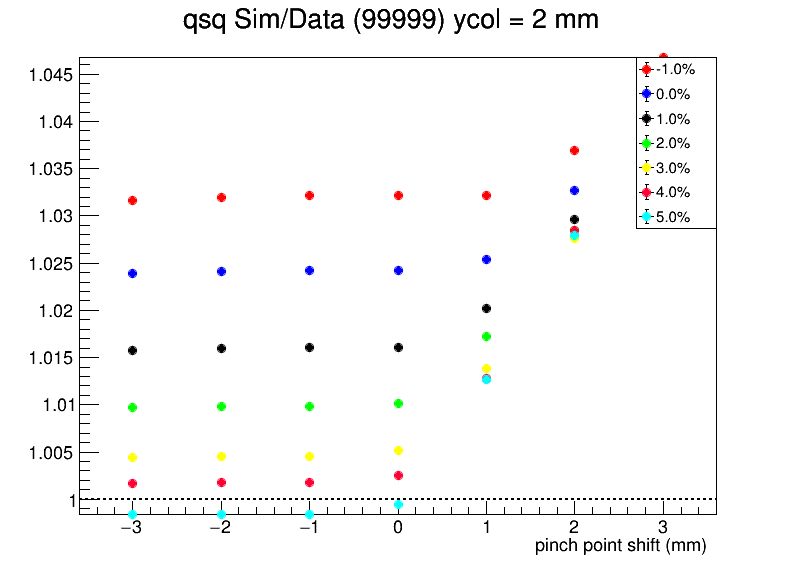
\includegraphics[width=0.32\linewidth]{pinch_scan_qsq_2_run99999}
    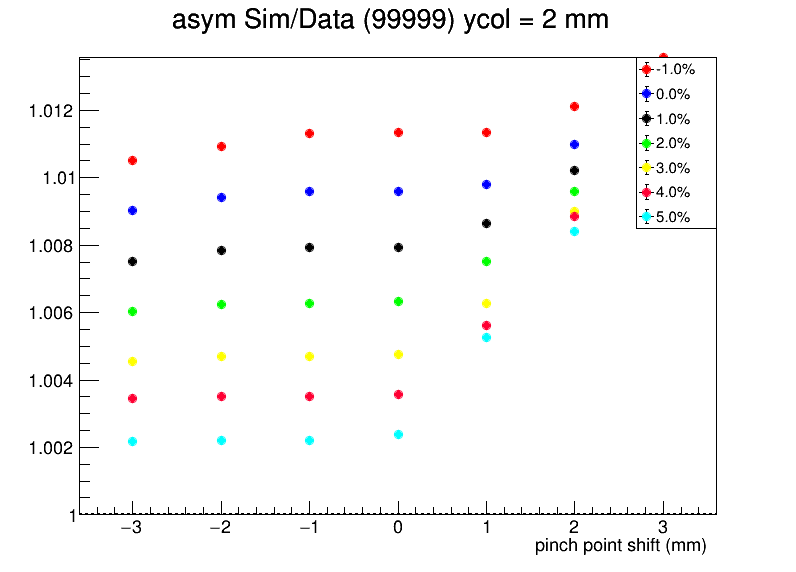
\includegraphics[width=0.32\linewidth]{pinch_scan_asym_2_run99999}
    \caption{Ratio of simulation to data average value for 
    $\theta_{lab}$, $Q^2$ and $\CA$. Top (bottom) row for left (right) arm.
    % FIXME: average over which runs?
    }
    \label{fig:pinch_scan}
\end{figure}

As shown in Fig. \ref{fig:pinch_scan}, when we shift the pinch point toward the
beam pipe (from negative values to positive values for left arm, opposite for 
right arm), the acceptance increases until the nominal value, and then saturates. 
Similar trend was seen for shift of Q1 collimator.
\begin{figure}[h!]
    \centering
    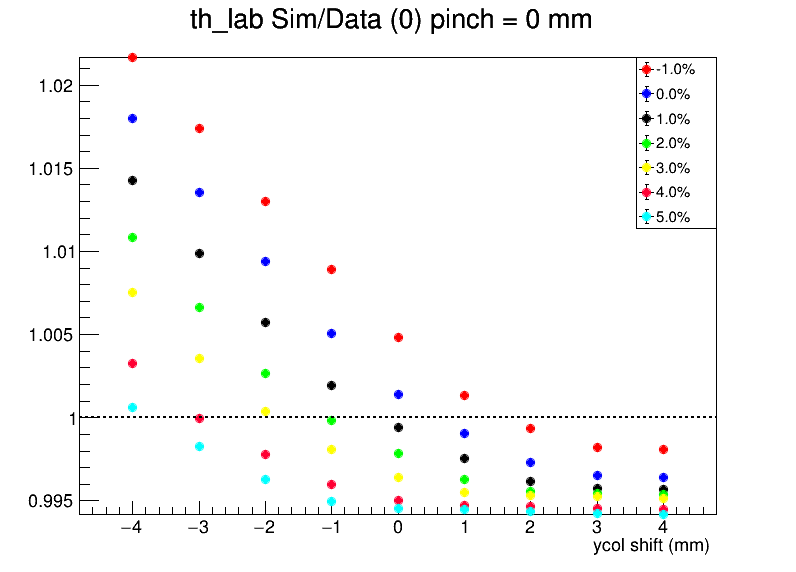
\includegraphics[width=0.49\linewidth]{col_scan_th_lab_0_run0}
    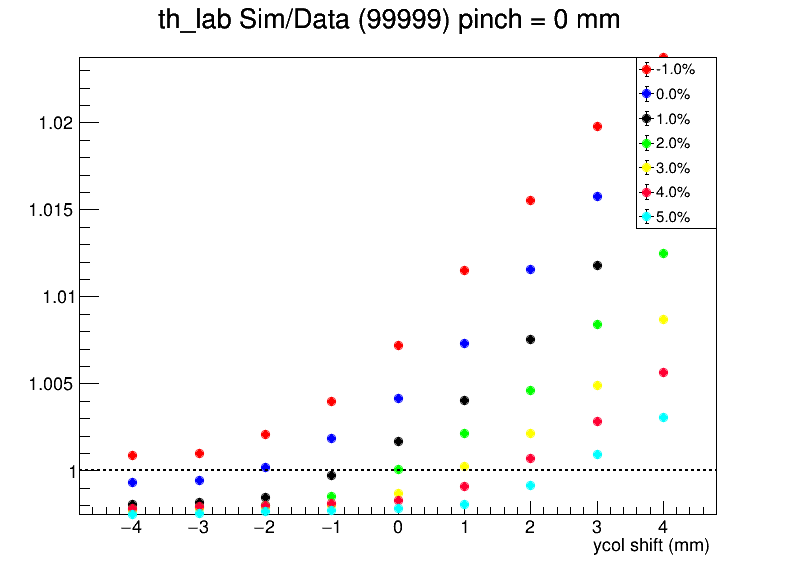
\includegraphics[width=0.49\linewidth]{col_scan_th_lab_0_run99999}
\end{figure}

Various correction was applied to the simulation values. That includes the position
difference between the production target and the calibration target, which was
$20\ mm$ downstream the production \Ca target; and the correction caused by
the database, which was optimized on one beam position ($x_0, y_0$):
\begin{equation}
    \phi_a = \phi_r + 0.5\ mrad/mm \times (x - x_0) + 0.5\ mrad/mm \times (y - y_0)
\end{equation}
(x, y) is the actual beam position. $\phi_a$ and $\phi_r$ are actual and reconstructed
$\phi_{tg}$. An extra acceptance was added to the right arm to get a better 
match.

From the ratio plot, we selected the best model which had the smallest difference
between simulation and data in $\theta_{lab}$ and $Q^2$:
\begin{table}[h!]
    \centering
    \begin{tabular}{c | c c c c}
	\hline
	    & septum & col shift ($mm$)	& pinch point shift ($mm$)	\\
	\hline
	LHRS	& +2\%	& -1	& 0 \\
	RHRS	& +5\%	& 2	& 0 \\
	\hline
    \end{tabular}
\end{table}

We can check the $\theta_{lab}$ for the best models
\begin{figure}[h!]
    \centering
    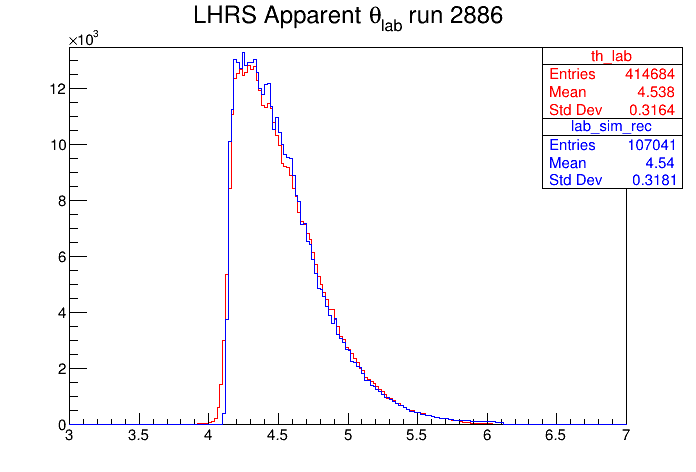
\includegraphics[width=0.49\linewidth]{best_model_run2886_th_lab}
    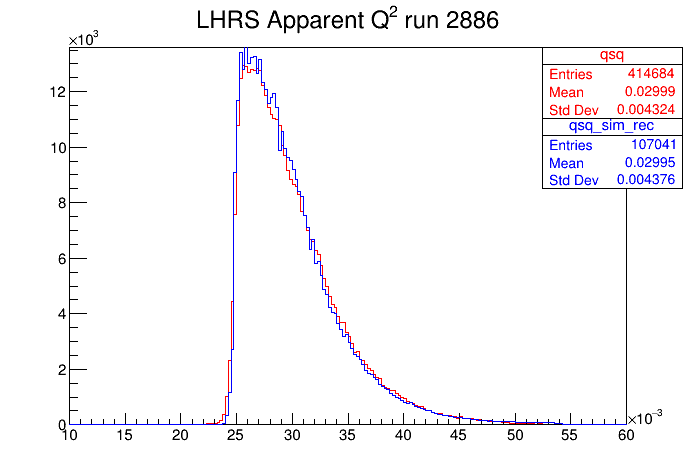
\includegraphics[width=0.49\linewidth]{best_model_run2886_qsq}
    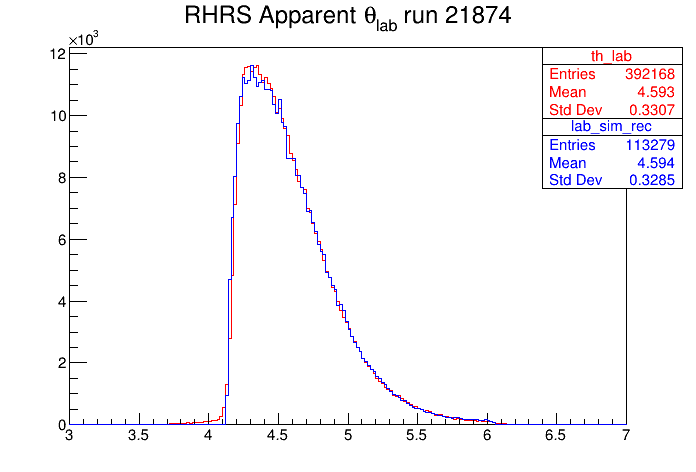
\includegraphics[width=0.49\linewidth]{best_model_run21874_th_lab}
    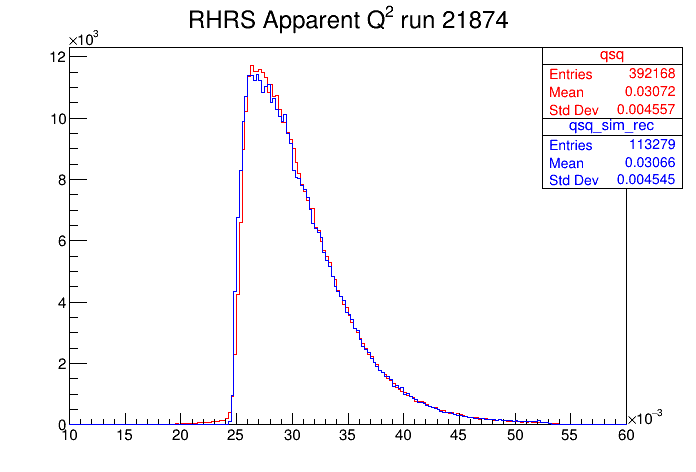
\includegraphics[width=0.49\linewidth]{best_model_run21874_qsq}
    \caption{$\theta_{lab}$ and $Q^2$ comparesion between best models and data (apparent values).}
\end{figure}
% We can also check the difference between the vertex values and data:
% \begin{figure}
%     \centering
%     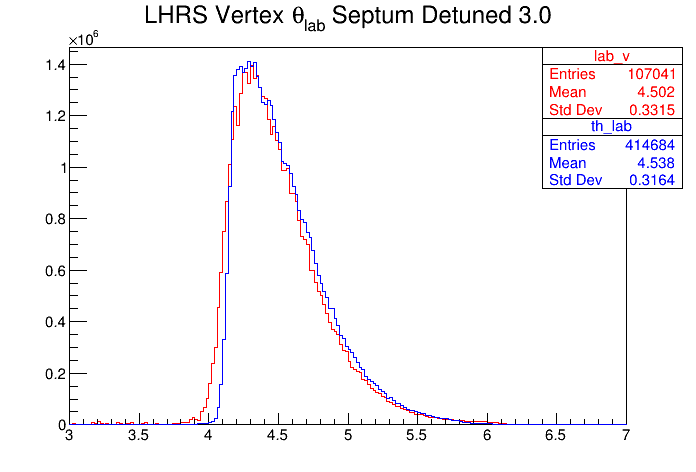
\includegraphics[width=0.49\linewidth]{p3_-2_0_0.0_run2886_th_lab_v}
%     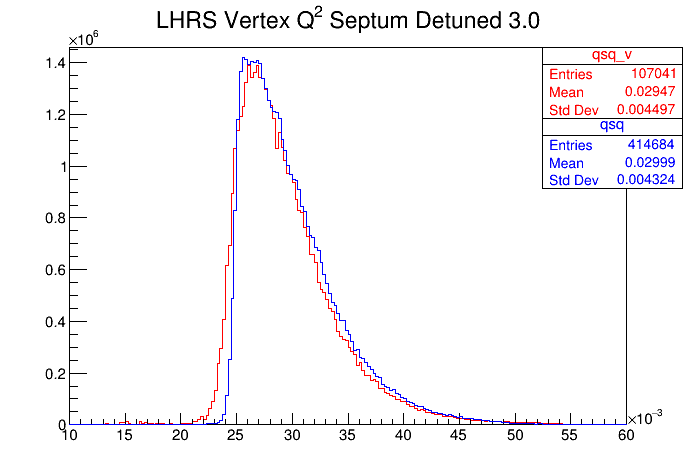
\includegraphics[width=0.49\linewidth]{p3_-2_0_0.0_run2886_qsq_v}
%     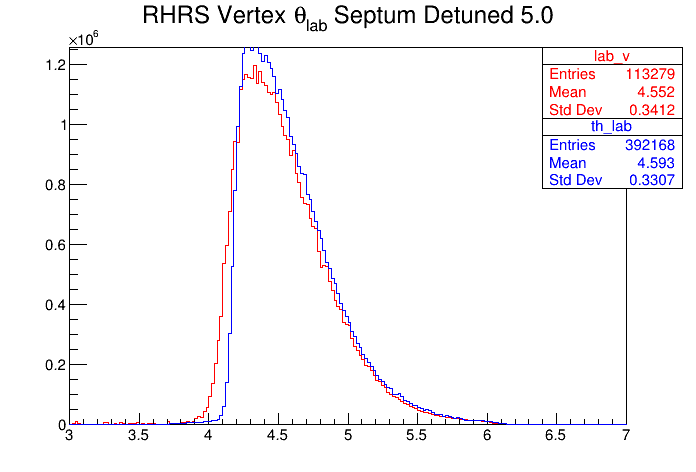
\includegraphics[width=0.49\linewidth]{p5_0_-1_0.0_run21874_th_lab_v}
%     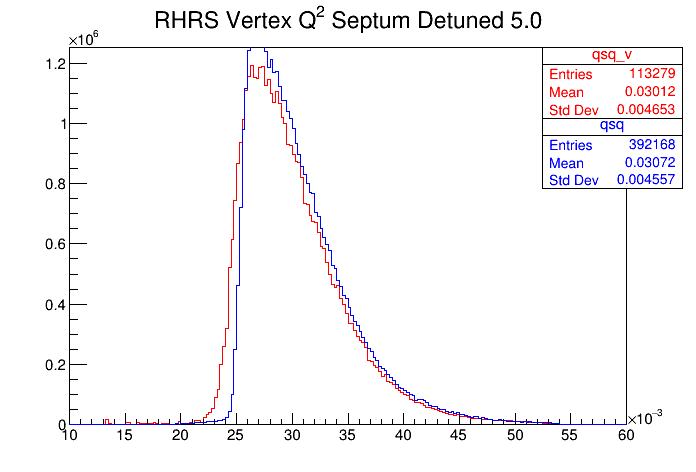
\includegraphics[width=0.49\linewidth]{p5_0_-1_0.0_run21874_qsq_v}
%     \caption{$\theta_{lab}$ and $Q^2$ comparesion between best models and data (apparent values).}
% \end{figure}

Using this best models, we can calculate the acceptance function as Eq. \ref{eq:acceptance_definition}:
\begin{figure}[h!]
    \centering
    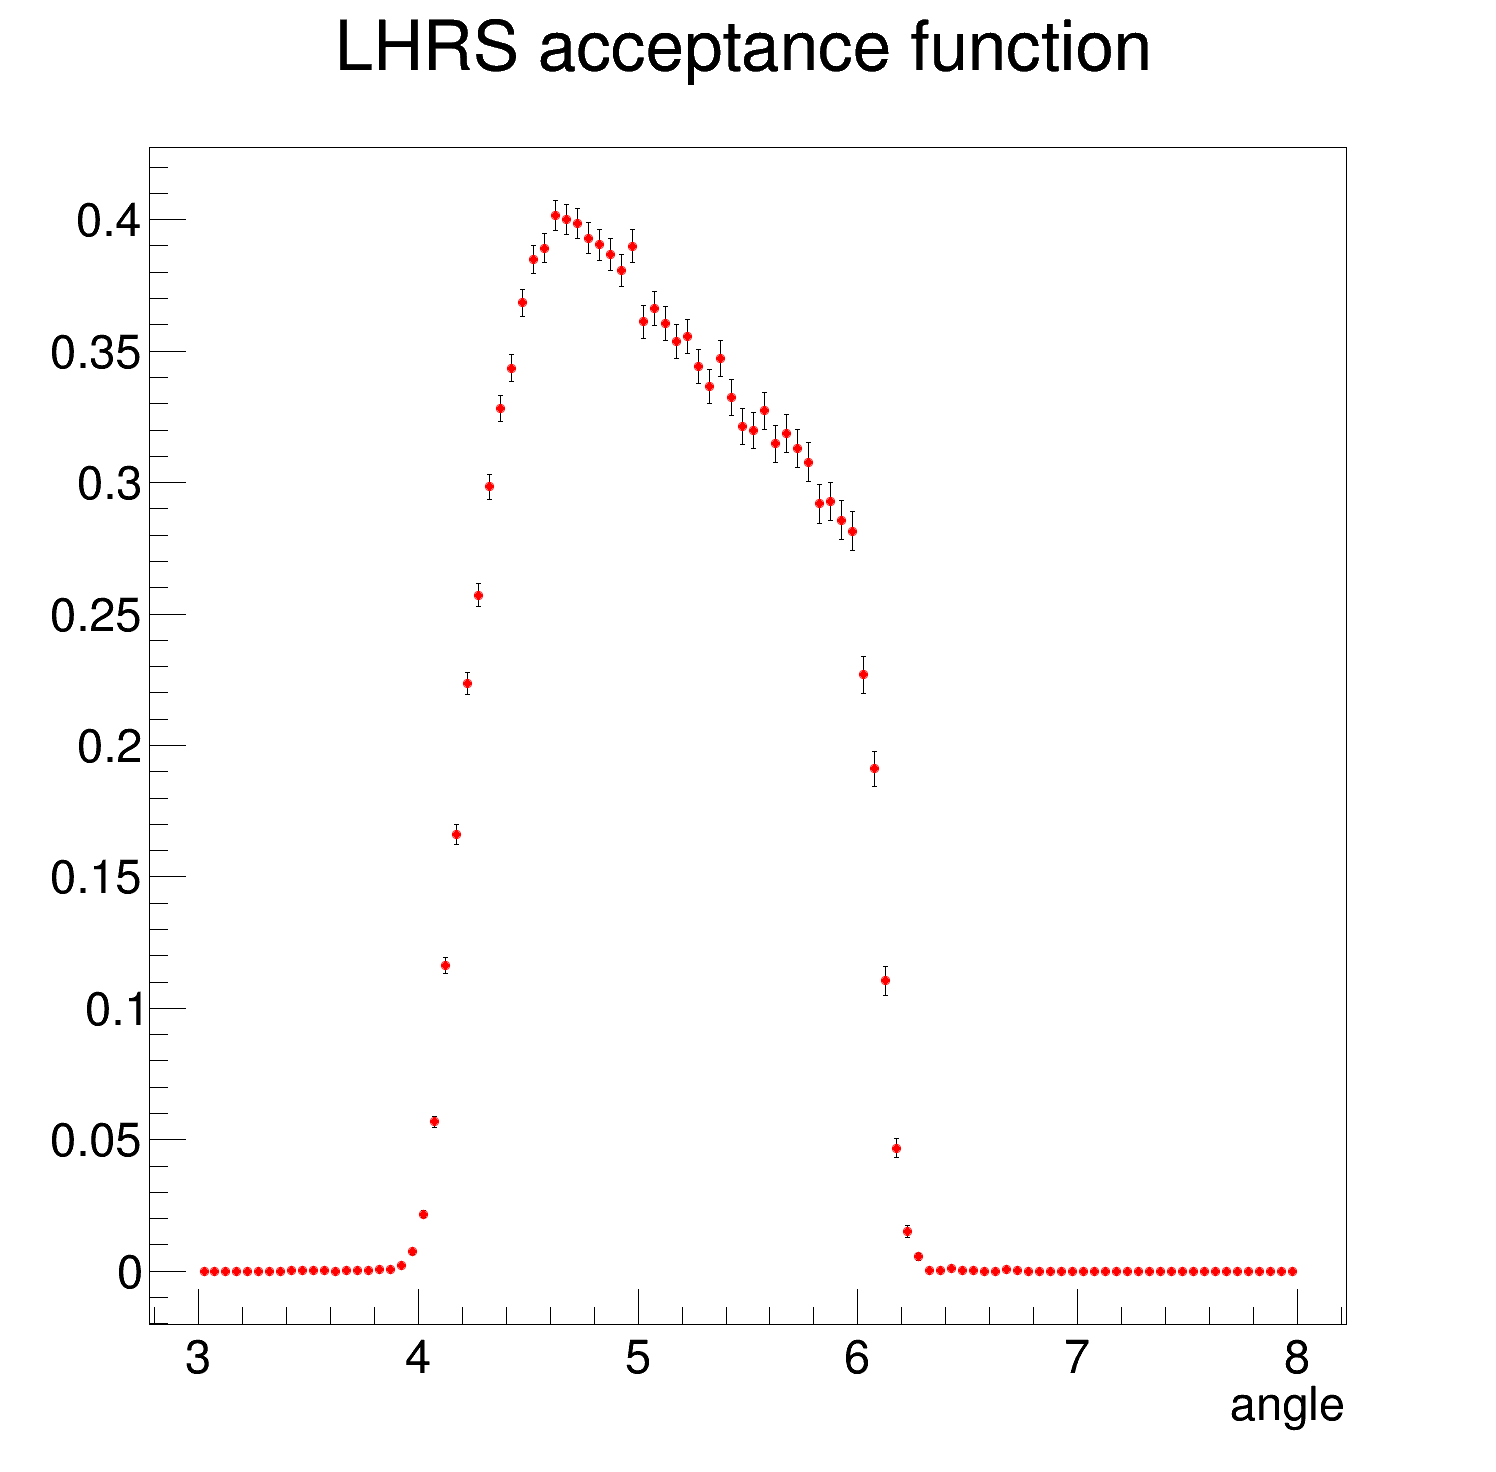
\includegraphics[width=0.49\linewidth]{acc1_L_p2_-1_0_0.0}
    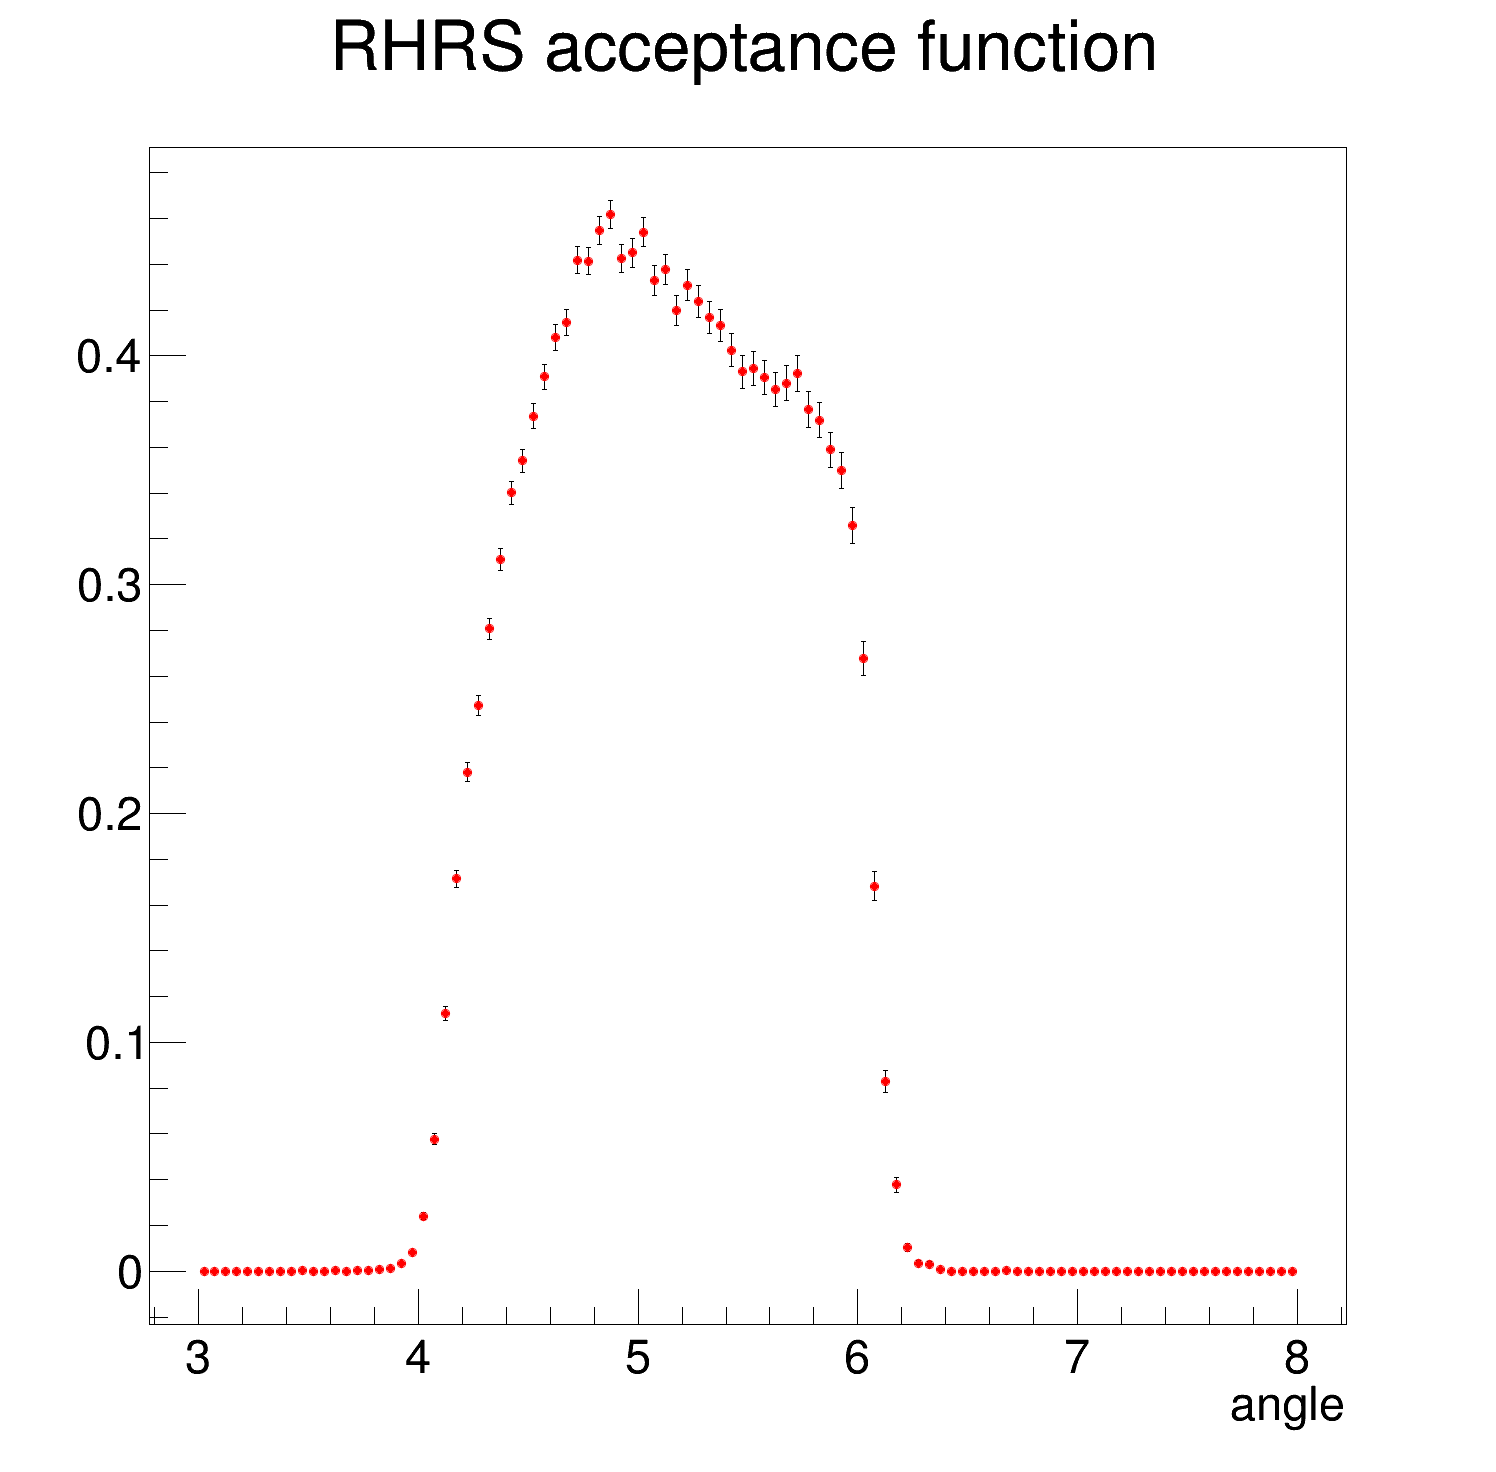
\includegraphics[width=0.49\linewidth]{acc1_R_p5_2_0_0.0}
    \caption{Acceptance function extraced using the best models.}
\end{figure}

% \subsection{tg variables}
